\documentclass[tikz]{standalone}
\usepackage{siunitx}
\usepackage[copies]{contour} % XeLaTeX-compatible text outlines
\usepackage{etoolbox,ifthen}
\usetikzlibrary{3d,angles,arrows,arrows.meta,calc,circuits.ee.IEC,decorations.markings,
  decorations.pathmorphing,fadings,patterns,quotes,shapes,shapes.multipart}

% 各卷共用的数学记号。课程专用记号见相应的主入口。
\RequirePackage{amsmath,amssymb,bm,upgreek}

% 数集与函数空间
\newcommand*{\NN}{\mathbb{N}}
\newcommand*{\ZZ}{\mathbb{Z}}
\newcommand*{\QQ}{\mathbb{Q}}
\newcommand*{\RR}{\mathbb{R}}
\newcommand*{\CC}{\mathbb{C}}
\newcommand*{\FF}{\mathbb{F}}
\newcommand*{\cont}{\mathcal{C}}  % 连续函数空间，\cont^k 表示 k 次连续可微
\newcommand*{\poly}{\mathcal{P}}  % \poly_n 中多项式的次数至多为 n

% 微分与常数。文本中的无点 i 和字母下加点另有明确的命令。
\NewCommandCopy{\dotlessi}{\i}
\NewCommandCopy{\dotbelow}{\d}
\renewcommand*{\i}{\mathrm{i}}
\newcommand*{\nd}{\mathrm{d}}
\renewcommand*{\d}{\mathop{}\!\mathrm{d}}
\newcommand*{\e}{\mathop{}\!\mathrm{e}}
\newcommand*{\const}{\mathrm{const}}
\newcommand*{\vd}{\mathop{}\!\delta}  % 变分、依赖过程的热量或功的微元
\newcommand*{\p}{\partial}
\newcommand{\dd}[2][]{\frac{\d^{#1}}{\nd{#2}^{#1}}}
\newcommand{\dv}[3][]{\frac{\d^{#1}#2}{\nd{#3}^{#1}}}
\newcommand{\pp}[2][]{\frac{\p^{#1}}{\p{#2}^{#1}}}
\newcommand{\pv}[3][]{\frac{\p^{#1}#2}{\p{#3}^{#1}}}
\newcommand{\pw}[3]{\frac{\p^2{#1}}{\p{#2}\p{#3}}}

% 函数与算符
\let\Re\relax
\let\Im\relax
\DeclareMathOperator{\Re}{Re}
\DeclareMathOperator{\Im}{Im}
\DeclareMathOperator{\sech}{sech}
\DeclareMathOperator{\csch}{csch}
\DeclareMathOperator{\sinc}{sinc}
\DeclareMathOperator{\sgn}{sgn}
\DeclareMathOperator{\id}{id}
\DeclareMathOperator{\PV}{PV}
\DeclareMathOperator{\FT}{\mathcal{F}}
\DeclareMathOperator{\Beta}{B}
\DeclareMathOperator*{\argmin}{arg\,min}
\DeclareMathOperator*{\argmax}{arg\,max}
\newcommand*{\bigo}{\mathcal{O}}
\newcommand*{\intR}{\int_{-\infty}^\infty}
\newcommand*{\intRplus}{\int_0^\infty}

% 矢量、线性代数与场算符
\newcommand*{\hatbm}[1]{\hat{\bm{#1}}} % 带帽的粗体符号，含义随卷定义
\newcommand*{\dotbm}[1]{\dot{\bm{#1}}}
\newcommand*{\uvec}[1]{\mathop{}\!\hatbm{#1}}  % 系数后自动留薄空；单独取负写 -{\uvec n}
\newcommand*{\grad}{\nabla}
\renewcommand*{\div}{\nabla\cdot}
\newcommand*{\curl}{\nabla\times}
\newcommand*{\laplacian}{\nabla^2}
\DeclareMathOperator{\rank}{rank}
\DeclareMathOperator{\diag}{diag}
\DeclareMathOperator{\tr}{tr}
\DeclareMathOperator{\Span}{span}
\DeclareMathOperator{\nullsp}{N}
\DeclareMathOperator{\colsp}{C}
\newcommand*{\transp}{^\top}
\newcommand*{\conj}{^\ast}
\newcommand*{\adjoint}{^\dagger}
\newcommand*{\inv}{^{-1}}

% 概率、统计与物理量
\renewcommand*{\P}{\operatorname{P}}  % 段落符号 ¶ 可用 \textparagraph
\DeclareMathOperator{\E}{E}
\DeclareMathOperator{\Var}{Var}
\DeclareMathOperator{\BinDist}{Bin}
\DeclareMathOperator{\NormalDist}{N}
\newcommand*{\avg}[1]{\overline{#1}}
\newcommand*{\NA}{N_{\mathrm{A}}}
\newcommand*{\kB}{k_{\mathrm{B}}}
\newcommand*{\muB}{\mu_{\mathrm{B}}}
\newcommand*{\Ek}{E_{\mathrm{k}}}
\newcommand*{\FWHM}{\mathrm{FWHM}}
\newcommand*{\electron}{\mathrm{e}}       % 粒子标签，如 m_\electron
\newcommand*{\proton}{\mathrm{p}}
\newcommand*{\nucleus}{\mathrm{N}}
\newcommand*{\excitedstate}{\mathrm{e}}
\newcommand*{\groundstate}{\mathrm{g}}
\newcommand*{\CM}{\mathrm{CM}}
\newcommand*{\transv}{\mathrm t}  % 横向分量或模式的标签
\newcommand*{\longit}{\mathrm l}  % 纵向分量或模式的标签
\newcommand*{\electric}{\mathrm e}
\newcommand*{\magnetic}{\mathrm m}
\newcommand*{\incident}{\mathrm i}
\newcommand*{\initial}{\mathrm i}
\newcommand*{\final}{\mathrm f}
\newcommand*{\hi}{\mathrm{hi}}
\newcommand*{\lo}{\mathrm{lo}}
\newcommand*{\eff}{\mathrm{eff}}
\newcommand*{\tot}{\mathrm{tot}}

% 括号与 Dirac 记号。显式声明让公式预览也能读到每个尺寸的命令。
\newcommand{\abs}[1]{\lvert#1\rvert}
\newcommand{\bigabs}[1]{\bigl\lvert#1\bigr\rvert}
\newcommand{\Bigabs}[1]{\Bigl\lvert#1\Bigr\rvert}
\newcommand{\biggabs}[1]{\biggl\lvert#1\biggr\rvert}
\newcommand{\Biggabs}[1]{\Biggl\lvert#1\Biggr\rvert}

\newcommand{\norm}[1]{\lVert#1\rVert}
\newcommand{\bignorm}[1]{\bigl\lVert#1\bigr\rVert}
\newcommand{\Bignorm}[1]{\Bigl\lVert#1\Bigr\rVert}
\newcommand{\biggnorm}[1]{\biggl\lVert#1\biggr\rVert}
\newcommand{\Biggnorm}[1]{\Biggl\lVert#1\Biggr\rVert}

\newcommand{\eval}[1]{{#1}\rvert}
\newcommand{\bigeval}[1]{{#1}\bigr\rvert}
\newcommand{\Bigeval}[1]{{#1}\Bigr\rvert}
\newcommand{\biggeval}[1]{{#1}\biggr\rvert}
\newcommand{\Biggeval}[1]{{#1}\Biggr\rvert}

\newcommand{\floor}[1]{\lfloor#1\rfloor}
\newcommand{\bigfloor}[1]{\bigl\lfloor#1\bigr\rfloor}
\newcommand{\Bigfloor}[1]{\Bigl\lfloor#1\Bigr\rfloor}
\newcommand{\biggfloor}[1]{\biggl\lfloor#1\biggr\rfloor}
\newcommand{\Biggfloor}[1]{\Biggl\lfloor#1\Biggr\rfloor}

\newcommand{\ceil}[1]{\lceil#1\rceil}
\newcommand{\bigceil}[1]{\bigl\lceil#1\bigr\rceil}
\newcommand{\Bigceil}[1]{\Bigl\lceil#1\Bigr\rceil}
\newcommand{\biggceil}[1]{\biggl\lceil#1\biggr\rceil}
\newcommand{\Biggceil}[1]{\Biggl\lceil#1\Biggr\rceil}

\newcommand{\ave}[1]{\langle#1\rangle}
\newcommand{\bigave}[1]{\bigl\langle#1\bigr\rangle}
\newcommand{\Bigave}[1]{\Bigl\langle#1\Bigr\rangle}
\newcommand{\biggave}[1]{\biggl\langle#1\biggr\rangle}
\newcommand{\Biggave}[1]{\Biggl\langle#1\Biggr\rangle}

\newcommand{\set}[2]{\{#1\,\vert\,#2\}}
\newcommand{\bigset}[2]{\bigl\{#1\,\big\vert\,#2\bigr\}}
\newcommand{\Bigset}[2]{\Bigl\{#1\,\Big\vert\,#2\Bigr\}}
\newcommand{\biggset}[2]{\biggl\{#1\,\bigg\vert\,#2\biggr\}}
\newcommand{\Biggset}[2]{\Biggl\{#1\,\Bigg\vert\,#2\Biggr\}}

\newcommand{\division}[2]{{#1}/{#2}}
\newcommand{\bigdivision}[2]{{#1}\big/{#2}}
\newcommand{\Bigdivision}[2]{{#1}\Big/{#2}}
\newcommand{\biggdivision}[2]{{#1}\bigg/{#2}}
\newcommand{\Biggdivision}[2]{{#1}\Bigg/{#2}}

\newcommand{\inp}[2]{\langle#1,#2\rangle}
\newcommand{\biginp}[2]{\bigl\langle#1,#2\bigr\rangle}
\newcommand{\Biginp}[2]{\Bigl\langle#1,#2\Bigr\rangle}
\newcommand{\bigginp}[2]{\biggl\langle#1,#2\biggr\rangle}
\newcommand{\Bigginp}[2]{\Biggl\langle#1,#2\Biggr\rangle}

\newcommand{\bra}[1]{\langle#1\rvert}
\newcommand{\bigbra}[1]{\bigl\langle#1\bigr\rvert}
\newcommand{\Bigbra}[1]{\Bigl\langle#1\Bigr\rvert}
\newcommand{\biggbra}[1]{\biggl\langle#1\biggr\rvert}
\newcommand{\Biggbra}[1]{\Biggl\langle#1\Biggr\rvert}

\newcommand{\ket}[1]{\lvert#1\rangle}
\newcommand{\bigket}[1]{\bigl\lvert#1\bigr\rangle}
\newcommand{\Bigket}[1]{\Bigl\lvert#1\Bigr\rangle}
\newcommand{\biggket}[1]{\biggl\lvert#1\biggr\rangle}
\newcommand{\Biggket}[1]{\Biggl\lvert#1\Biggr\rangle}

\newcommand{\braket}[2]{\langle#1\vert#2\rangle}
\newcommand{\bigbraket}[2]{\bigl\langle#1\big\vert#2\bigr\rangle}
\newcommand{\Bigbraket}[2]{\Bigl\langle#1\Big\vert#2\Bigr\rangle}
\newcommand{\biggbraket}[2]{\biggl\langle#1\bigg\vert#2\biggr\rangle}
\newcommand{\Biggbraket}[2]{\Biggl\langle#1\Bigg\vert#2\Biggr\rangle}

\newcommand{\mel}[3]{\langle#1\vert#2\vert#3\rangle}
\newcommand{\bigmel}[3]{\bigl\langle#1\big\vert#2\big\vert#3\bigr\rangle}
\newcommand{\Bigmel}[3]{\Bigl\langle#1\Big\vert#2\Big\vert#3\Bigr\rangle}
\newcommand{\biggmel}[3]{\biggl\langle#1\bigg\vert#2\bigg\vert#3\biggr\rangle}
\newcommand{\Biggmel}[3]{\Biggl\langle#1\Bigg\vert#2\Bigg\vert#3\Biggr\rangle}

\newcommand{\ketbra}[2]{\lvert#1\rangle\langle#2\rvert}
\newcommand{\bigketbra}[2]{\bigl\lvert#1\bigr\rangle\bigl\langle#2\bigr\rvert}
\newcommand{\Bigketbra}[2]{\Bigl\lvert#1\Bigr\rangle\Bigl\langle#2\Bigr\rvert}
\newcommand{\biggketbra}[2]{\biggl\lvert#1\biggr\rangle\biggl\langle#2\biggr\rvert}
\newcommand{\Biggketbra}[2]{\Biggl\lvert#1\Biggr\rangle\Biggl\langle#2\Biggr\rvert}

% 兼容旧版笔记中的内积与外积命令。
\let\brkt\braket
\let\bigbrkt\bigbraket
\let\Bigbrkt\Bigbraket
\let\biggbrkt\biggbraket
\let\Biggbrkt\Biggbraket
\let\ktbr\ketbra
\let\bigktbr\bigketbra
\let\Bigktbr\Bigketbra
\let\biggktbr\biggketbra
\let\Biggktbr\Biggketbra

\newcommand{\bigp}[1]{\bigl(#1\bigr)}
\newcommand{\Bigp}[1]{\Bigl(#1\Bigr)}
\newcommand{\biggp}[1]{\biggl(#1\biggr)}
\newcommand{\Biggp}[1]{\Biggl(#1\Biggr)}

\newcommand{\bigb}[1]{\bigl[#1\bigr]}
\newcommand{\Bigb}[1]{\Bigl[#1\Bigr]}
\newcommand{\biggb}[1]{\biggl[#1\biggr]}
\newcommand{\Biggb}[1]{\Biggl[#1\Biggr]}

\newcommand{\bigB}[1]{\bigl\{#1\bigr\}}
\newcommand{\BigB}[1]{\Bigl\{#1\Bigr\}}
\newcommand{\biggB}[1]{\biggl\{#1\biggr\}}
\newcommand{\BiggB}[1]{\Biggl\{#1\Biggr\}}

% 公式排版
% 方程组的内容是一个 aligned 块，左花括号随整组方程的高度伸展。
\newcommand{\eqnset}[1]{\left\{#1\right.}
\newcommand{\fracdisp}[2]{\frac{\displaystyle #1}{\displaystyle #2}}
\newcommand*{\vs}{\mathord{\text{–}}}
\newcommand*{\otherwise}{\text{otherwise}}
\newcommand*{\qqquad}{\qquad\quad}
\newcommand*{\qqqquad}{\qquad\qquad}

\renewcommand*{\le}{\leqslant}
\renewcommand*{\leq}{\leqslant}
\renewcommand*{\ge}{\geqslant}
\renewcommand*{\geq}{\geqslant}

% 界面上的入射波、反射波和透射波。正文与图册采用相同下标。
\newcommand*{\reflected}{\mathrm r}
\newcommand*{\transmitted}{\mathrm t}


\begin{tikzfadingfrompicture}[name=interference]
  \def\lambd{0.5} % wavelength
  \foreach \r in {1,...,15}
    \foreach \j in {1,...,25}
       \path [line width=\lambd*\j,draw=transparent!0,opacity=0.04]
          (0,0) circle (\lambd*\r); %(0:\r) arc (0:180:\r);
\end{tikzfadingfrompicture}

\begin{document}

% Fields and waves
\begingroup
\tikzset{>=latex}
\tikzset{->-/.style={decoration={
  markings,
  mark=at position .5 with {\arrow{>}}},postaction={decorate}}}
\tikzset{-<-/.style={decoration={
  markings,
  mark=at position .5 with {\arrow{<}}},postaction={decorate}}}


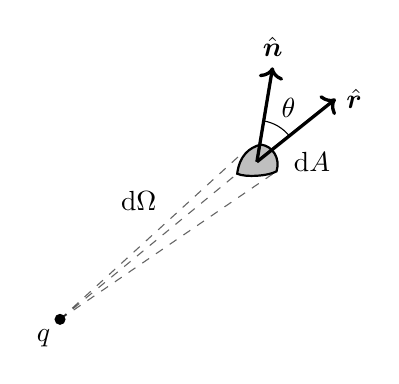
\begin{tikzpicture}
    \fill(0,0) circle (2pt) node[below left]{$q$};

    \coordinate (P) at (2.5, 2);
    \coordinate (n) at (2.7, 3.2);
    \coordinate (r) at (3.5, 2.8);

    \draw[fill=gray!50, thick, shift={(P)}]
        (-0.25,-0.15) .. controls (-0.15,-0.2) and (0.15,-0.18) ..
        (0.25,-0.12) .. controls (0.3,0.05) and (0.2,0.2) ..
        (0.05,0.22) .. controls (-0.1,0.18) and (-0.22,0.08) ..
        (-0.25,-0.15) -- cycle;
    \node at (P) [xshift=0.7cm] {$\d A$};

    \draw[->, very thick] (P) -- (r) node[right]{$\uvec{r}$};
    \draw[->, very thick] (P) -- (n) node[above]{$\uvec{n}$};

    \pic["$\theta$", draw, angle radius=15, angle eccentricity=1.5]{angle=r--P--n};

    \draw[dashed, opacity=0.6] (0,0) -- ($(P)+(-0.25,-0.15)$);
    \draw[dashed, opacity=0.6] (0,0) -- ($(P)+(0.25,-0.12)$);
    % \draw[dashed, opacity=0.6] (0,0) -- ($(P)+(0.05,0.22)$);
    \draw[dashed, opacity=0.6] (0,0) -- ($(P)+(-0.22,0.08)$);

    \node at (1, 1.5) {$\d\Omega$};
    \label{gauss-law}
\end{tikzpicture}

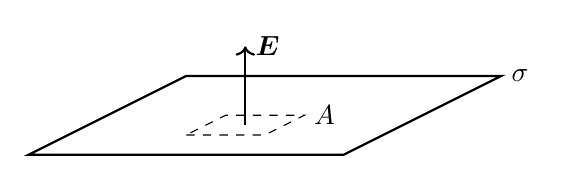
\begin{tikzpicture}
    \draw[thick](0, 0)--(4, 0)--(6, 1)node[right]{$\sigma$}--(2, 1)--cycle;
    \draw[dashed, shift={(2, 0.25)}](0, 0)--(1, 0)--(1.5, .25)node[right]{$A$}--(.5, .25)--cycle;
    % \draw[shift={(2, 0.35)}](0, 0)--(1, 0)--(1.5, .25)--(.5, .25)--cycle;
    % \draw[dashed, shift={(2, 0.15)}](0, 0)--(1, 0)--(1.5, .25)--(.5, .25)--cycle;
    \draw[thick, ->, shift={(2.75, 0.375)}](0, 0)--(0, 1)node[right]{$\bm E$};
    \label{e-of-plane}
\end{tikzpicture}

\begin{tikzpicture}
    \draw[thick](-3, 0)--(3, 0)node[right]{$\lambda$};
    \draw[dashed, yshift=.2cm](-.5, 0)--(.5, 0);
    \draw[dashed, yshift=-.2cm](-.5, 0)--(.5, 0);
    \draw[dashed](.5, 0)ellipse(.1 and .2);
    \draw[dashed](-.5, 0)ellipse(.1 and .2);
    \draw[thick, ->, yshift=.2cm](0, 0)--(0, 1)node[right]{$\bm E$};
    \label{e-of-line}
\end{tikzpicture}

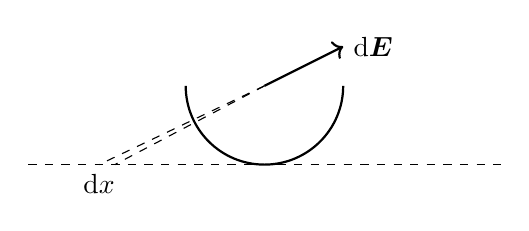
\begin{tikzpicture}
    \draw[thick](-1, 0)arc(-180:0:1);
    \draw[dashed](-3, -1)--(3, -1);
    \draw[dashed](0, 0)--(-2-.1, -1)node[below]{$\d x$};
    \draw[dashed](0, 0)--(-2+.1, -1);
    \draw[thick, ->](0, 0)--(1, .5)node[right]{$\d\bm E$};
    \label{e-of-half-circle}
\end{tikzpicture}

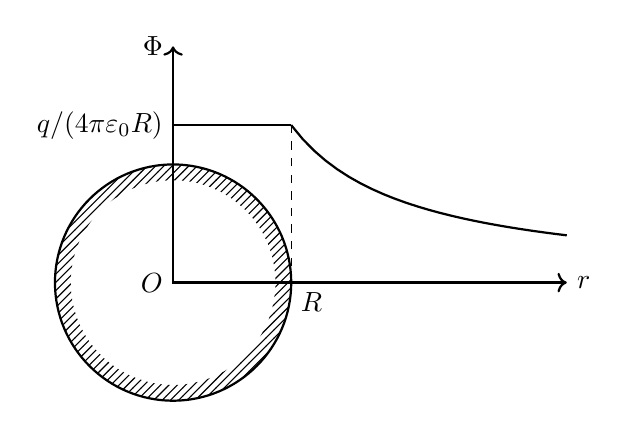
\begin{tikzpicture}[even odd rule]
    \fill[pattern=north east lines](0, 0)circle(1.3)(0, 0)circle(1.5);
    \draw[thick](0, 0)node[left]{$O$}circle(1.5);
    \draw[thick, <->](0, 3)node[left]{$\Phi$}--(0, 0)--(5, 0)node[right]{$r$};
    \draw[dashed](1.5, 0)node[below right]{$R$}--(1.5, 2);
    \draw[thick](0, 2)node[left]{$q/(4\pi\varepsilon_0R)$}--(1.5, 2);
    \draw[thick, domain=1.5:5]plot(\x, {3/\x});
    \label{phi-of-sphere-conductor}
\end{tikzpicture}

\begin{tikzpicture}
    \draw[thick](-3, 0)node[below right]{1}node[above right]{2}--(3, 0)node[right]{$\sigma$};
    \draw[thick, ->](0, 0)--(0, 1)node[right]{$\uvec{n}$};
    \draw[dashed](0, 2)--(0, -2);
    \draw[thick, ->](-2, -1)node[left]{$\bm E_1$}--(0, 0);
    \draw[thick, ->](0, 0)--(2, 1.5)node[right]{$\bm E_2$};
    \label{e-between-surfaces}
\end{tikzpicture}

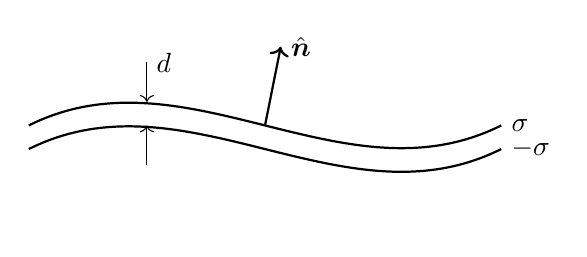
\begin{tikzpicture}[xscale=2]
    \draw[thick](0, 0).. controls (1, 1) and (2, -1) .. (3, 0)node[right]{$\sigma$};
    \draw[thick, yshift=-.3cm](0, 0).. controls (1, 1) and (2, -1) .. (3, 0)node[right]{$-\sigma$};
    \draw[->, shift={(.75, 0)}](0, -.5)--(0, 0);
    \draw[->, shift={(.75, .3)}](0, .5)node[right]{$d$}--(0, 0);
    \draw[thick, ->, xshift=1.5cm](0, 0)--(.1, 1)node[right]{$\uvec{n}$};
    \label{dipole-layers}
\end{tikzpicture}

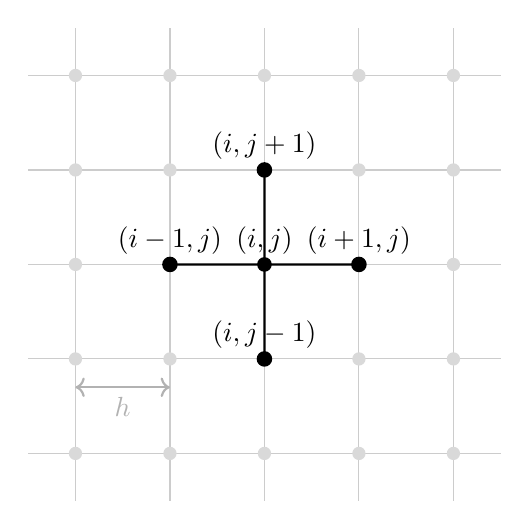
\begin{tikzpicture}[scale=1.2]
    \draw[gray!40, thin] (-2.5, -2.5) grid (2.5, 2.5);
    \foreach \i in {-2, -1, 0, 1, 2} {
        \foreach \j in {-2, -1, 0, 1, 2} {
            \fill[gray!30] (\i,\j) circle (2pt);
        }
    }
    \coordinate (O) at (0, 0) node [above] {$(i, j)$} circle (2.2pt) [fill=black];
    \draw[thick] (O)--(-1, 0) node [above] {$(i-1,j)$} circle (2pt) [fill=black];
    \draw[thick] (O)--(1, 0) node [above] {$(i+1,j)$} circle (2pt) [fill=black];
    \draw[thick] (O)--(0, 1) node [above] {$(i,j+1)$} circle (2pt) [fill=black];
    \draw[thick] (O)--(0, -1) node [above] {$(i,j-1)$} circle (2pt) [fill=black];
    \draw[<->, thick, gray!60] (-2, -1.3) -- (-1, -1.3) node [midway, below] {$h$};
    \label{finite-difference-method}
\end{tikzpicture}

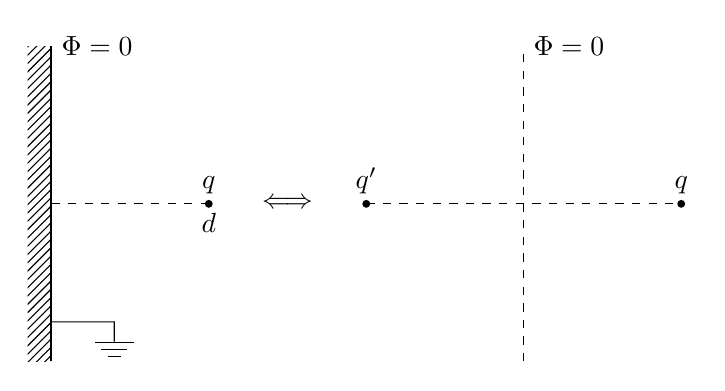
\begin{tikzpicture}[circuit ee IEC]
    \begin{scope}
        \fill[pattern=north east lines](-.3, 0)rectangle(0, 4);
        \draw[thick](0, 0)--(0, 4)node[right]{$\Phi = 0$};
        \draw (0, 0.5) to (0.8, 0.5) to [ground={at end}] (0.8, 0.15);
        \draw[dashed](0, 2)--(2, 2)node[below]{$d$};
        \fill[black](2, 2)circle(.05)node[above]{$q$};
    \end{scope}
    \node at (3, 2) {$\iff$};
    \begin{scope}[xshift=6cm]
        \draw[dashed](0, 0)--(0, 4)node[right]{$\Phi = 0$};
        \draw[dashed](-2, 2)--(2, 2);
        \fill[black](2, 2)circle(.05)node[above]{$q$};
        \fill[black](-2, 2)circle(.05)node[above]{$q'$};
    \end{scope}
    \label{method-of-images-plane}
\end{tikzpicture}

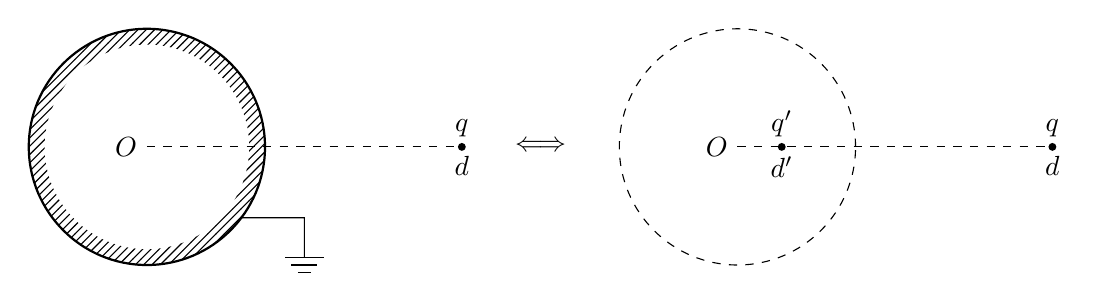
\begin{tikzpicture}[circuit ee IEC]
    \begin{scope}
        \fill[even odd rule, pattern=north east lines](0, 0)circle(1.5)(0, 0)circle(1.3);
        \draw[thick](0, 0)circle(1.5);
        \draw (1.2, -.9) to (2, -.9) to [ground={at end}] (2, -1.5);
        \draw[dashed](0, 0)node[left]{$O$}--(4, 0);
        \fill[black](4, 0)circle(.05)node[below]{$d$}node[above]{$q$};
    \end{scope}
    \node at (5, 0) {$\iff$};
    \begin{scope}[xshift=7.5cm]
        \draw[dashed](0, 0)circle(1.5);
        \draw[dashed](0, 0)node[left]{$O$}--(4, 0);
        \fill[black](4, 0)circle(.05)node[below]{$d$}node[above]{$q$};
        \fill[black](.5625, 0)circle(.05)node[below]{$d'$}node[above]{$q'$};
    \end{scope}
    \label{method-of-images-sphere}
\end{tikzpicture}

\begin{tikzpicture}
    \draw[loosely dash dot](-5, 0)--(5, 0);
    \fill[black](4, 0)circle(.05)node[above]{$-Q$}node[below]{$+R$};
    \fill[black](-4, 0)circle(.05)node[above]{$+Q$}node[below]{$-R$};
    \draw[dashed](-4, 0)--(0, .8)--(4, 0);
    %\draw[thick, <->](1, 1)--(0, .8)--(1, .6);
    \draw[thick, ->](0, .8)--(2, .8)node[above]{$\bm E_0$};
    \label{uniform-e-approx-pm-q}
\end{tikzpicture}

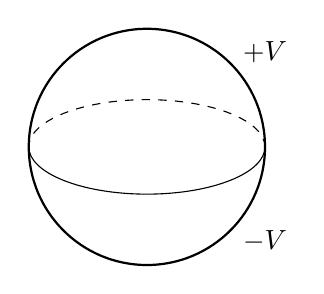
\begin{tikzpicture}[scale=.6]
    \draw[thick](0, 0)circle(2.5);
    \draw[dashed](2.5, 0)arc(0:180:2.5 and 1);
    \draw(-2.5, 0)arc(-180:0:2.5 and 1);
    \node at(2.5, 2){$+V$};
    \node at(2.5, -2){$-V$};
    \label{2-hemisphere}
\end{tikzpicture}

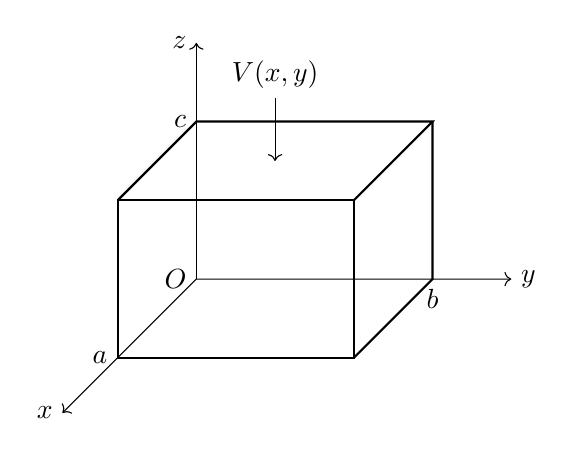
\begin{tikzpicture}
    \draw[thick](0, 0)node[left]{$a$}rectangle(3, 2);
    \draw[thick](0, 2)--(1, 3)node[left]{$c$}--(4, 3)--(3, 2);
    \draw[thick](4, 3)--(4, 1)node[below]{$b$}--(3, 0);
    \draw[<->](5, 1)node[right]{$y$}--(1, 1)node[left]{$O$}--(-.7, -.7)node[left]{$x$};
    \draw[->](1, 1)--(1, 4)node[left]{$z$};
    \draw[->](2, 3.3)node[above]{$V(x,y)$}--(2, 2.5);
    \label{3d-rectangular-box}
\end{tikzpicture}

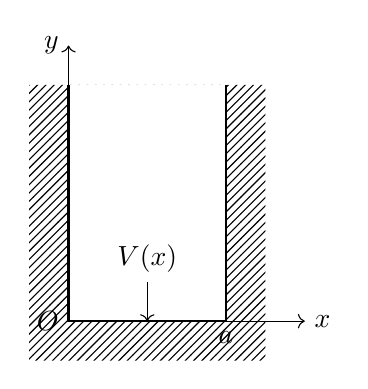
\begin{tikzpicture}[even odd rule]
    \coordinate (O) at (0, 0);
    \fill[pattern=north east lines](-.5, -.5)rectangle(2.5, 3)(O)rectangle(2, 3);
    \draw[<->](3, 0)node[right]{$x$}--(O)node[left]{$O$}--(0, 3.5)node[left]{$y$};
    \draw[thick](0, 3)--(O)--(2, 0)node[below]{$a$}--(2, 3);
    \draw[<-](1, 0)--(1, 0.5)node[above]{$V(x)$};
    \label{2d-rectangular-hole}
\end{tikzpicture}

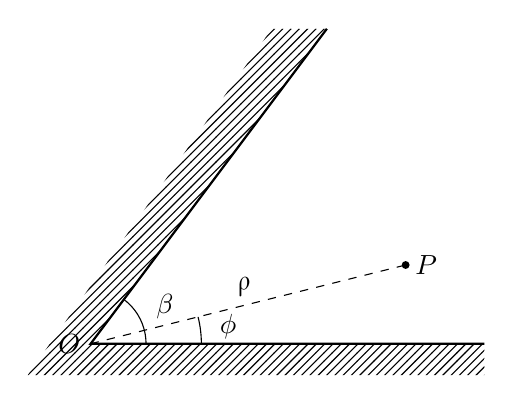
\begin{tikzpicture}
    \coordinate (o) at (0, 0);
    \coordinate (p) at (4, 1);
    \coordinate (a) at (5, 0);
    \coordinate (b) at (3, 4);
    \fill[pattern=north east lines](2.3, 4)--(b)--(o)--(a)--(5, -.4)--(-.8, -.4);
    \draw[thick](b)--(o)node[left]{$O$}--(a);
    \draw[dashed](o)--(p)node[right]{$P$}node[midway, above, sloped]{$\rho$};
    \fill(p)circle(.05);
    \pic[draw, angle radius=20, angle eccentricity=1.5, "$\beta$"]{angle=a--o--b};
    \pic[draw, angle radius=40, angle eccentricity=1.25, "$\phi$"]{angle=a--o--p};
    \label{2d-angular-boundary}
\end{tikzpicture}

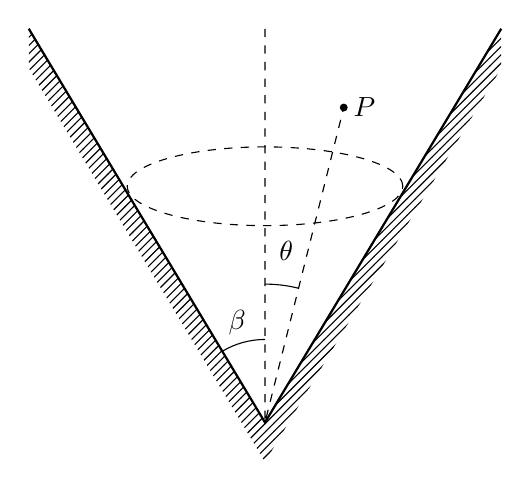
\begin{tikzpicture}
    \coordinate (o) at (0, 0);
    \coordinate (z) at (0, 5);
    \coordinate (a) at (3, 5);
    \coordinate (b) at (-3, 5);
    \coordinate (p) at (1, 4);
    \fill[pattern=north east lines](b)--(o)--(a)--(3, 4.5)--(0, -.5)--(-3, 4.5);
    \draw[thick](a)--(o)--(b);
    \draw[dashed](z)--(o)--(p);
    \draw[dashed](0, 3)ellipse(1.75 and .5);
    \fill(p)circle(.05)node[right]{$P$};
    \pic[draw, angle radius=30, angle eccentricity=1.25, "$\beta$"]{angle=z--o--b};
    \pic[draw, angle radius=50, angle eccentricity=1.25, "$\theta$"]{angle=p--o--z};
    \label{2d-conical-boundary}
\end{tikzpicture}

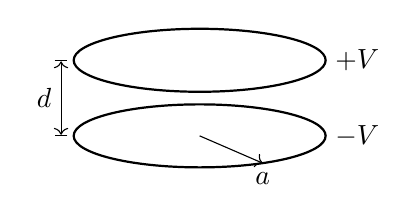
\begin{tikzpicture}[scale=.8]
    \draw[thick](0, 0)ellipse(2 and .5);
    \node[right] at (2, 0) {$-V$};
    \draw[thick](0, 1.2)ellipse(2 and .5);
    \node[right] at (2, 1.2) {$+V$};
    \draw[->](0, 0)--(1, -.433)node[below]{$a$};
    \draw[|<->|](-2.2, 0)--(-2.2, 1.2)node[midway, left]{$d$};
    \label{circular-disk-capacitor}
\end{tikzpicture}

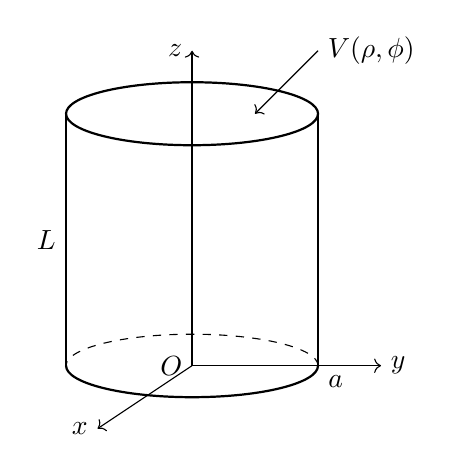
\begin{tikzpicture}[scale=.8]
    \draw[<->](0, 5)node[left]{$z$}--(0, 0)node[left]{$O$}--(3, 0)node[right]{$y$};
    \draw[->](0, 0)--(-1.5, -1)node[left]{$x$};
    \draw[dashed](2, 0)arc(0:180:2 and .5);
    \draw[thick](-2, 0)arc(-180:0:2 and .5);
    \draw[thick](0, 4)ellipse(2 and .5);
    \draw[thick](2, 0)node[below right]{$a$}--(2, 4);
    \draw[thick](-2, 0)--(-2, 4)node[midway, left]{$L$};
    \draw[<-](1, 4)--(2, 5)node[right]{$V(\rho,\phi)$};
    \label{cylindrical-boundary}
\end{tikzpicture}

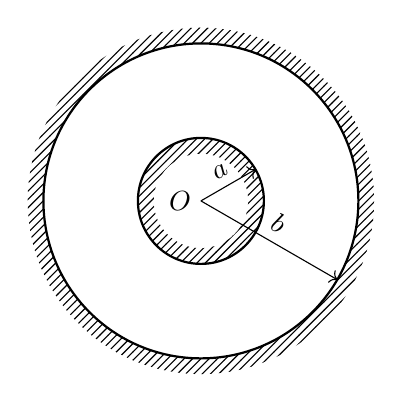
\begin{tikzpicture}[even odd rule]
    \coordinate[label=left:$O$](O)at(0, 0);
    \fill[pattern=north east lines](O)circle(2.2)(O)circle(2)(O)circle(.8)(O)circle(.6);
    \draw[thick](O)circle(.8)(O)circle(2);
    \draw[->](O)--(30:.8)node[midway, sloped, above]{$a$};
    \draw[->](O)--(-30:2)node[midway, sloped, above]{$b$};
    \label{concentric-spheres-boundary}
\end{tikzpicture}

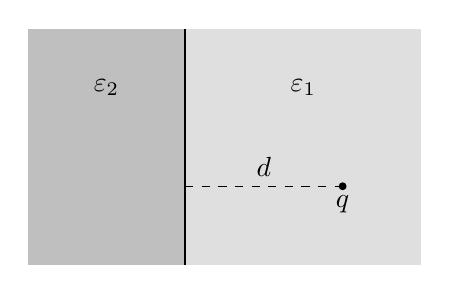
\begin{tikzpicture}
    \fill[gray!25](0, 0)rectangle(3, 3);
    \fill[gray!50](0, 0)rectangle(-2, 3);
    \node at(1.5, 2.25){$\varepsilon_1$};
    \node at(-1, 2.25){$\varepsilon_2$};
    \draw[thick](0, 0)--(0, 3);
    \draw[dashed](0, 1)--(2, 1)node[midway, above]{$d$};
    \fill[black](2, 1)circle(.05)node[below]{$q$};
    \label{method-of-images-dielectrics}
\end{tikzpicture}

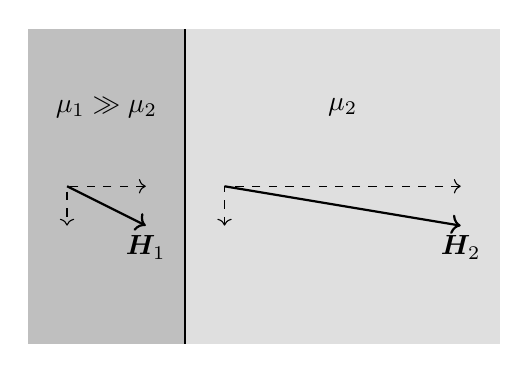
\begin{tikzpicture}
    \fill[gray!25](0, 0)rectangle(4, 4);
    \fill[gray!50](0, 0)rectangle(-2, 4);
    \node at(-1, 3){$\mu_1 \gg \mu_2$};
    \node at(2, 3){$\mu_2$};
    \draw[thick](0, 0)--(0, 4);
    \draw[dashed, <->](-.5, 2)--(-1.5, 2)--(-1.5, 1.5);
    \draw[thick, ->](-1.5, 2)--(-.5, 1.5)node[below]{$\bm H_1$};
    \draw[dashed, <->](3.5, 2)--(.5, 2)--(.5, 1.5);
    \draw[thick, ->](.5, 2)--(3.5, 1.5)node[below]{$\bm H_2$};
    \label{h-between-magnetic-surfaces}
\end{tikzpicture}

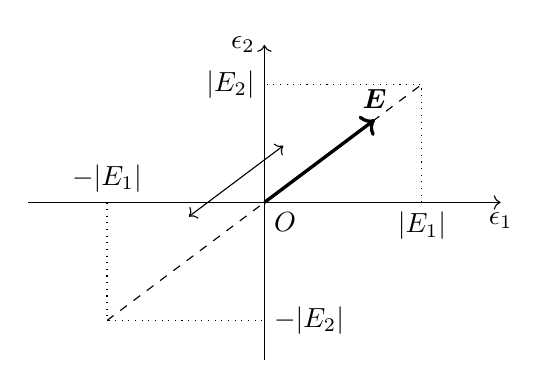
\begin{tikzpicture}
    \coordinate(O)at(0, 0);
    \coordinate(x)at(3, 0);
    \coordinate(y)at(0, 2);
    \coordinate(E)at(2, 1.5);
    \draw[->](-3, 0)--(x)node[below]{$\epsilon_1$};
    \draw[->](0, -2)--(y)node[left]{$\epsilon_2$};
    \node[below right]at(O){$O$};
    \draw[dashed](-2, -1.5)--(E);
    \draw[dotted](-2, 0)node[above]{$-\abs{E_1}$}--(-2, -1.5)--(0, -1.5)node[right]{$-\abs{E_2}$};
    \draw[dotted](2, 0)node[below]{$\abs{E_1}$}--(E)--(0, 1.5)node[left]{$\abs{E_2}$};
    \draw[very thick, ->, scale=0.7](O)--(2, 1.5)node[above]{$\bm E$};
    \draw[<->, scale=0.3, shift={(-1.2, 0.9)}](-2, -1.5)--(2, 1.5);
    % \pic[draw, angle radius=15, angle eccentricity=1.5, "$\delta$"]{angle=x--O--E};
    \label{linear-polarization}
\end{tikzpicture}

\begin{tikzpicture}[scale=.8]
    \draw[->](-3, 0)--(3, 0)node[below]{$\epsilon_1$};
    \draw[->](0, -3)--(0, 3)node[left]{$\epsilon_2$};
    \draw[dashed](0, 0)node[above left]{$O$}circle(2);
    \node[below]at(2, 0) {$\abs{E_1}$};
    \draw[very thick, ->](0, 0)--(45:2)node[above]{$\bm E$};
    \draw[->](30:2.6)arc(30:60:2.6);
    \label{circular-polarization}
\end{tikzpicture}

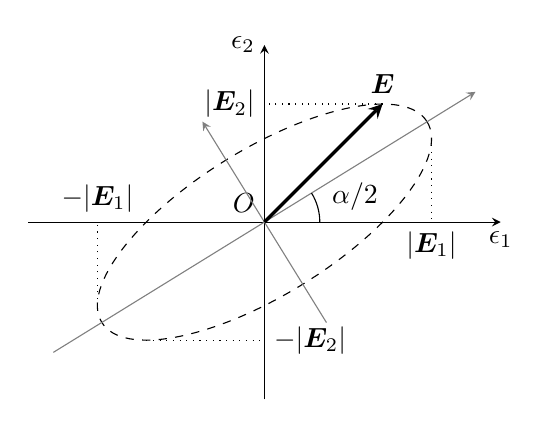
\begin{tikzpicture}[scale=1.5, >=stealth]
    \coordinate(O)at(0, 0);
    \coordinate(x)at(2, 0);
    \coordinate(a)at(31.68:2.5);
    \draw[->](-2, 0)--(x)node[below]{$\epsilon_1$};
    \draw[->](0, -1.5)--(0, 1.5)node[left]{$\epsilon_2$};
    \node[above left]at(O){$O$};
    \draw[dashed, rotate=31.68](O)ellipse[x radius=1.618, y radius=.618];
    \draw[->, gray, rotate=31.68](-2.1, 0)--(2.1, 0);
    \draw[->, gray, rotate=31.68](0, -1)--(0, 1);
    \draw[dotted](1.414, .707)--(1.414, 0)node[below]{$\abs{\bm E_1}$};
    \draw[dotted](-1.414, -.707)--(-1.414, 0)node[above]{$-\abs{\bm E_1}$};
    \draw[dotted](1, 1)--(0, 1)node[left]{$\abs{\bm E_2}$};
    \draw[dotted](-1, -1)--(0, -1)node[right]{$-\abs{\bm E_2}$};
    \draw[very thick, ->](0, 0)--(1, 1)node[above]{$\bm E$};
    \pic[draw, angle radius=20, angle eccentricity=1.7, "$\alpha/2$"]{angle=x--O--a};
    \label{elliptical-polarization}
\end{tikzpicture}

\begin{tikzpicture}
    \coordinate(O)at(0, 0);
    \coordinate(n)at(0, 1);
    \coordinate(u)at(0, -1);
    \coordinate(i)at(-2, 2);
    \coordinate(r)at(2, 2);
    \coordinate(t)at(1.2, -2);
    \fill[gray!8](-3, 0)rectangle(3, 2);
    \fill[gray!50](-3, 0)rectangle(3, -2);
    \draw(-3, 0)node[above right]{$n_\incident$}node[below right]{$n_\transmitted$}--(3, 0);
    \draw[dashed](O)--(u);
    \draw[->](O)--(n)node[above]{$\uvec{n}$};
    \draw[thick, ->-](O)--(r)node[midway, right]{$\bm k_\reflected$};
    \draw[thick, ->-](i)--(O)node[midway, left]{$\bm k_\incident$};
    \draw[thick, ->-](O)--(t)node[midway, right]{$\bm k_\transmitted$};
    \pic["$\theta_\incident$", draw, angle radius=20, angle eccentricity=1.5]{angle=n--O--i};
    \pic["$\theta_\reflected$", draw, angle radius=20, angle eccentricity=1.5]{angle=r--O--n};
    \pic["$\theta_\transmitted$", draw, angle radius=20, angle eccentricity=1.5]{angle=u--O--t};
    \label{reflection-and-transmission}
\end{tikzpicture}

\begin{tikzpicture}
    \fill[gray!8](-3, 0)rectangle(3, 2);
    \fill[gray!50](-3, 0)rectangle(3, -2);
    \draw(-3, 0)node[above right]{$n_1$}node[below right]{$n_2$}--(3, 0);
    \draw[dashed](n)--(u);
    \draw[thick, ->-](i)--(O)node[midway, below left]{$1$};
    \draw[thick, ->-](O)--(r)node[midway, below right]{$r_{12}$};
    \draw[thick, ->-](O)--(t)node[midway, above right]{$t_{12}$};
    \label{stokes-relations-i}
\end{tikzpicture}

\begin{tikzpicture}
    \coordinate(tr)at(-1.2, -2);
    \fill[gray!8](-3, 0)rectangle(3, 2);
    \fill[gray!50](-3, 0)rectangle(3, -2);
    \draw(-3, 0)node[above right]{$n_1$}node[below right]{$n_2$}--(3, 0);
    \draw[dashed](n)--(u);
    \draw[thick, ->-, red](r)--(O)node[midway, below right]{$r_{12}$};
    \draw[thick, ->-, red]([shift={(-.1, 0)}]O)--([shift={(-.1, 0)}]i)node[midway, below left]{$r_{12}^2$};
    \draw[dashed, ->-, red]([shift={(-.1, 0)}]O)--([shift={(-.1, 0)}]tr)node[midway, above left]{$r_{12}t_{12}$};
    \draw[thick, ->-, blue](t)--(O)node[midway, above right]{$t_{12}$};
    \draw[thick, ->-, blue](O)--(i)node[midway, above right]{$t_{12}t_{21}$};
    \draw[dashed, ->-, blue](O)--(tr)node[midway, below right]{$t_{12}r_{21}$};
    \label{stokes-relations-ii}
\end{tikzpicture}

\begin{tikzpicture}
    \coordinate(t)at(1.5, -2.5);
    \coordinate(Ei)at(-1.2, 1.2);
    \coordinate(Er)at(1, 1);
    \coordinate(Et)at(.6, -1);
    \fill[gray!8](-3, 0)rectangle(3, 2);
    \fill[gray!50](-3, 0)rectangle(3, -2.5);
    \draw(-3, 0)node[above right]{$n_\incident$}node[below right]{$n_\transmitted$}--(3, 0);
    \draw[dashed](n)--(u);
    \draw(O)--(r);
    \draw(i)--(O);
    \draw(O)--(t);
    % incident
    \draw[thick, ->](Ei)--(-.7, .7)node[shift={(30:.3)}]{$\bm k_\incident$};
    \draw[thick, ->](Ei)--(-1.7, .7)node[left]{$\bm H_\incident$};
    \draw[thick, fill=white](Ei)circle(.12)node[shift={(30:.4)}]{$\bm E_\incident$};
    \fill[black](Ei)circle(.06);
    % reflect
    \draw[thick, ->](Er)--(1.5, 1.5)node[shift={(150:.3)}]{$\bm k_\reflected$};
    \draw[thick, ->](Er)--(1.5, .5)node[right]{$\bm H_\reflected$};
    \draw[thick, fill=white](Er)circle(.12)node[shift={(150:.4)}]{$\bm E_\reflected$};
    \fill[black](Er)circle(.06);
    % transmit
    \draw[thick, ->](Et)--(1.2, -2)node[right]{$\bm k_\transmitted$};
    \draw[thick, ->](Et)--(.1, -1.3)node[left]{$\bm H_\transmitted\!$};
    \draw[thick, fill=white](Et)circle(.12)node[right]{$\bm E_\transmitted$};
    \fill[black](Et)circle(.06);
    \label{senkrecht-polarization}
\end{tikzpicture}

\begin{tikzpicture}
    \fill[gray!8](-3, 0)rectangle(3, 2);
    \fill[gray!50](-3, 0)rectangle(3, -2.5);
    \draw(-3, 0)node[above right]{$n_\incident$}node[below right]{$n_\transmitted$}--(3, 0);
    \draw[dashed](n)--(u);
    \draw(O)--(r);
    \draw(i)--(O);
    \draw(O)--(t);
    % incident
    \draw[thick, ->](Ei)--(-.7, .7)node[shift={(30:.3)}]{$\bm k_\incident$};
    \draw[thick, ->](Ei)--(-.7, 1.7)node[right]{$\bm E_\incident$};
    \draw[thick, fill=white](Ei)circle(.12)node[shift={(210:.4)}]{$\bm H_\incident$};
    \fill[black](Ei)circle(.06);
    % reflect
    \draw[thick, ->](Er)--(1.5, 1.5)node[shift={(-30:.3)}]{$\bm k_\reflected$};
    \draw[thick, ->](Er)--(.5, 1.5)node[shift={(150:.3)}]{$\bm E_\reflected$};
    \draw[thick, fill=white](Er)circle(.12)node[shift={(-30:.4)}]{$\bm H_\reflected$};
    \fill[black](Er)circle(.06);
    % transmit
    \draw[thick, ->](Et)--(1.2, -2)node[right]{$\bm k_\transmitted$};
    \draw[thick, ->](Et)--(1.1, -.7)node[right]{$\bm E_\transmitted$};
    \draw[thick, fill=white](Et)circle(.12)node[shift={(210:.4)}]{$\bm H_\transmitted$};
    \fill[black](Et)circle(.06);
    \label{parallel-polarization}
\end{tikzpicture}

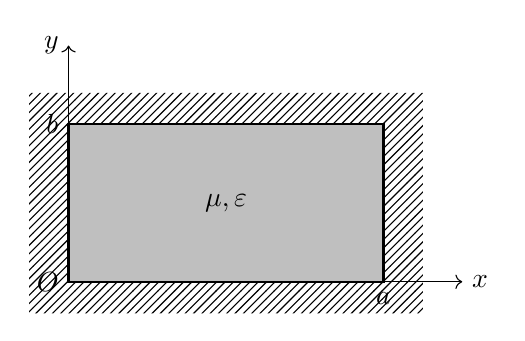
\begin{tikzpicture}[even odd rule]
    \fill[pattern=north east lines](-.5, -.4)rectangle(4.5, 2.4)(0, 0)rectangle(4, 2);
    \draw[thick, fill=gray!50](4, 0)node[below]{$a$}rectangle(0, 2)node[left]{$b$};
    \node at (2, 1) {$\mu,\varepsilon$};
    \draw[<->](0, 3)node[left]{$y$}--(0, 0)node[left]{$O$}--(5, 0)node[right]{$x$};
    \label{rectangular-waveguide}
\end{tikzpicture}

\begin{tikzpicture}[even odd rule]
    \coordinate(x)at(2, 0);
    \coordinate(P)at(60:1.5);
    \fill[pattern=north east lines](O)circle(2)(O)circle(2.2);
    \draw[thick, fill=gray!50](O)circle(2);
    \node at (0, -1) {$\mu,\varepsilon$};
    \draw[dashed](O)--(x)node[midway, below]{$a$};
    % \draw(O)--(P)node[midway, left]{$\rho$};
    % \pic["$\phi$", draw, angle radius=20, angle eccentricity=1.5]{angle=x--O--P};
    \label{circle-waveguide}
\end{tikzpicture}

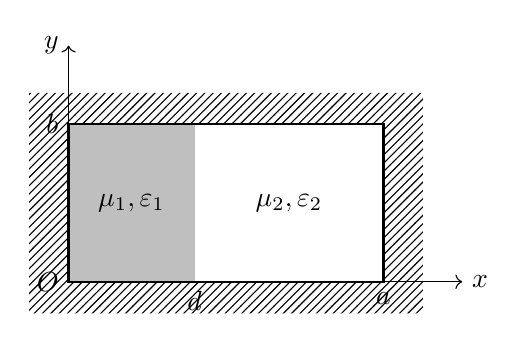
\begin{tikzpicture}[even odd rule]
    \fill[pattern=north east lines](-.5, -.4)rectangle(4.5, 2.4)(0, 0)rectangle(4, 2);
    \fill[gray!50](0, 0)rectangle(1.6, 2);
    \node at (1.6, 0) [below] {$d$};
    \draw[thick](4, 0)node[below]{$a$}rectangle(0, 2)node[left]{$b$};
    \node at (0.8, 1) {$\mu_1,\varepsilon_1$};
    \node at (2.8, 1) {$\mu_2,\varepsilon_2$};
    \draw[<->](0, 3)node[left]{$y$}--(0, 0)node[left]{$O$}--(5, 0)node[right]{$x$};
    \label{dielectric-waveguide}
\end{tikzpicture}

\begin{tikzpicture}[scale=1.2]
    \draw[->-](0, 0)--(2, 0)node[shift={(-.35, -.15)}]{$O$};
    \draw[thick,dashed](2-.5, -.5)--(2.5, .5)node[above right]{BS};
    \draw[->-](2, 0)--(5, 0)node[midway, below]{$c - u$};
    \draw[-<-](2.1, .1)--(5, .1)node[midway, above]{$c + u$};
    \fill[pattern=north east lines](5, .5)rectangle(5.2, -.5);
    \draw[thick](5, -.5)--(5, .5)node[above]{M$_1$};
    \draw[->-](2, 0)--(2, 3)node[midway, left]{$\sqrt{c^2 - u^2}$};
    \draw[-<-](2.1, .1)--(2.1, 3);
    \fill[pattern=north east lines](1.5, 3)rectangle(2.5, 3.2);
    \draw[thick](1.5, 3)--(2.5, 3)node[right]{M$_2$};
    \draw[->-](2.1,.1)--(2.1,-1.08);
    \node[draw,anchor=north] at (2.1,-1.08) {$\mathrm D$};
    \draw[<-](3.5, 1.5)--(4.5, 1.5)node[midway, below]{$u$}node[midway, above]{ether wind};
    \label{michelson-morley-experiment}
\end{tikzpicture}

\begin{tikzpicture}
    \coordinate (O) at (0, 0);
    \coordinate (x) at (3, 0);
    \coordinate (v) at (3, 2);
    \coordinate (e) at (2, -2);
    \draw[->, thick, gray, decorate, decoration={
        snake, amplitude=.4mm, segment length=2mm, post length=1mm}]
        (-3, 0)node[above]{$h\nu$}--(O);
    \draw[->, thick, decorate, decoration={
        snake, amplitude=.4mm, segment length=4mm, post length=1mm}]
        (O)--(v)node[right]{$h\nu'$};
    \draw[->, thick](O)--(e)node[right]{e$^-$};
    \draw[dashed](O)--(x);
    \pic[draw, "$\theta$", angle radius=8mm, angle eccentricity=1.2]{angle=x--O--v};
    \pic[draw, "$\phi$", angle radius=10mm, angle eccentricity=1.2]{angle=e--O--x};
    \label{compton-scattering}
\end{tikzpicture}

\begin{tikzpicture}[xscale=.8]
    \draw[->, thick](-3, 2.3)node[left]{$\lambda_+$}--(-2, 2.3)node[right]{$\bm v_+$};
    \draw[->, thick](3, 1.7)node[right]{$\lambda_-$}--(2, 1.7)node[left]{$\bm v_-$};
    \draw[thick](-3, 2)--(3, 2);
    \draw[dashed](0, 0)--(0, 2)node[midway, right]{$r$};
    \draw[->, thick](0, 0)--(.5, 0)node[above]{$\bm u$};
    \fill[black](0, 0)circle(0.1)node[left]{$q$};
    \label{q-in-lab-frame}
\end{tikzpicture}

\begin{tikzpicture}[xscale=.8]
    \draw[->, thick](-3, 2.3)node[left]{$\lambda_+'$}--(-2.2, 2.3)node[right]{$\bm v_+'$};
    \draw[->, thick](3, 1.7)node[right]{$\lambda_-'$}--(1.8, 1.7)node[left]{$\bm v_-'$};
    \draw[thick](-3, 2)--(3, 2);
    \draw[dashed](0, 0)--(0, 2)node[midway, right]{$r$};
    \fill[black](0, 0)circle(0.1)node[left]{$q$};
    \label{q-in-q-frame}
\end{tikzpicture}

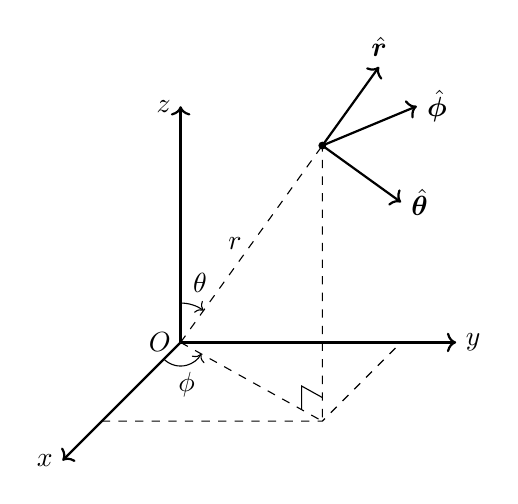
\begin{tikzpicture}
    \coordinate[label=left:$O$] (O) at (0, 0);
    \coordinate[label=left:$x$] (x) at (-1.5, -1.5);
    \coordinate[label=right:$y$] (y) at (3.5, 0);
    \coordinate[label=left:$z$] (z) at (0, 3);
    \coordinate (P) at (1.8, 2.5);
    \coordinate (Q) at (1.8, -1);
    \draw[thick, ->](O)--(y);
    \draw[thick, ->](O)--(z);
    \draw[thick, ->](O)--(x);
    \draw[dashed](O)--(P)node[midway, left]{$r$};
    \draw[thick, ->](P)--(2.52, 3.5)node[above]{$\uvec{r}$};
    \draw[thick, ->](P)--(3, 3)node[right]{$\uvec{\phi}$};
    \draw[thick, ->](P)--(2.8, 1.78)node[right]{$\uvec{\theta}$};
    \draw[dashed](O)--(Q)--(P);
    \fill[black](P)circle(0.05);
    \draw[dashed](-1, -1)--(Q)--(2.8, 0);
    \pic[draw, angle radius=3mm]{right angle=P--Q--O};
    \pic[draw, angle radius=5mm, angle eccentricity=1.6, <-, "$\theta$"]{angle=P--O--z};
    \pic[draw, angle radius=3mm, angle eccentricity=1.8, ->, "$\phi$"]{angle=x--O--Q};
    \label{spherical-coordinate}
\end{tikzpicture}

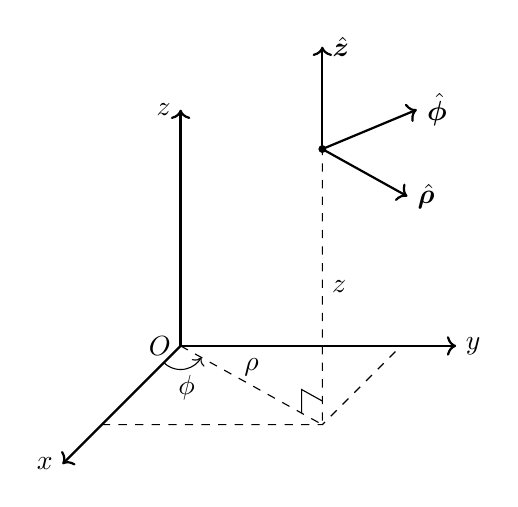
\begin{tikzpicture}
    \coordinate[label=left:$O$] (O) at (0, 0);
    \coordinate[label=left:$x$] (x) at (-1.5, -1.5);
    \coordinate[label=right:$y$] (y) at (3.5, 0);
    \coordinate[label=left:$z$] (z) at (0, 3);
    \coordinate (P) at (1.8, 2.5);
    \coordinate (Q) at (1.8, -1);
    \draw[thick, ->](O)--(y);
    \draw[thick, ->](O)--(z);
    \draw[thick, ->](O)--(x);
    \draw[thick, ->](P)--(2.88, 1.9)node[right]{$\uvec{\rho}$};
    \draw[thick, ->](P)--(3, 3)node[right]{$\uvec{\phi}$};
    \draw[thick, ->](P)--(1.8, 3.8)node[right]{$\uvec{z}$};
    \draw[dashed](O)--(Q)node[midway, above]{$\rho$}--(P)node[midway, right]{$z$};
    \fill[black](P)circle(0.05);
    \draw[dashed](-1, -1)--(Q)--(2.8, 0);
    \pic[draw, angle radius=3mm]{right angle=P--Q--O};
    \pic[draw, angle radius=3mm, angle eccentricity=1.8, ->, "$\phi$"]{angle=x--O--Q};
    \label{cylindrical-coordinate}
\end{tikzpicture}
\endgroup

% Birefringence
\begingroup
\standaloneconfig{border=3pt}
% ref: https://tikz.net/birefringence/
% author: Alexandros Tsagkaropoulos

% Drawing

%Notation

% Tikz Library

% Styles
%% Node Style in Order Text to Get Center Alignment
\tikzset{every text node part/.style={align=center}}
%% Main Ray Style
\tikzset{ray/.style = {postaction=decorate,decoration={markings,
						 mark=at position .49 with \arrow{stealth},
						 mark=between positions 0.1 and 0.4 step 0.5cm with {
						 \draw[fill=red, draw = red] circle[radius=1pt];
						 \draw[red, {Latex[length=1.3mm, width=1.5mm]}-{Latex[length=1.3mm, width=1.5mm]}] (0,-7pt) -- (0,7pt);},
						 mark=between positions 0.6 and 0.9 step 0.5cm with {
						 \draw[fill=red, draw = red] circle[radius=1pt];
						 \draw[red, {Latex[length=1.3mm, width=1.5mm]}-{Latex[length=1.3mm, width=1.5mm]}] (0,-7pt) -- (0,7pt);}
                                                        }
						 }
		}
%% Bottom Ray Inside Box
\tikzset{rayE1/.style = {postaction=decorate,decoration={markings,
						 mark=at position .52 with \arrow{stealth},
						 mark=between positions 0.65 and 0.9 step 0.7cm with {
						 \draw[red, {Latex[length=1.3mm, width=1.5mm]}-{Latex[length=1.3mm, width=1.5mm]}] (0,-7pt) -- (0,7pt);
						 \draw[fill=black!10, draw = black!10] circle[radius=1pt];}
                                                        }
						 }
		}
%% Bottom Ray Outside Box
\tikzset{rayE2/.style = {postaction=decorate,decoration={markings,
						 mark=at position .52 with \arrow{stealth},
						 mark=between positions 0.1 and 0.4 step 0.54cm with {
						 \draw[red, {Latex[length=1.3mm, width=1.5mm]}-{Latex[length=1.3mm, width=1.5mm]}] (0,-7pt) -- (0,7pt);
						 \draw[fill=white, draw = white] circle[radius=1pt];},
						 mark=between positions 0.6 and 0.9 step 0.5cm with {
						 \draw[red, {Latex[length=1.3mm, width=1.5mm]}-{Latex[length=1.3mm, width=1.5mm]}] (0,-7pt) -- (0,7pt);
						 \draw[fill=white, draw = white] circle[radius=1pt];}
                                                        }
						 }
		}
%% Upper Ray Inside Box
\tikzset{rayT1/.style = {postaction=decorate,decoration={markings,
						 mark=at position .52 with \arrow{stealth},
						 mark=between positions 0.65 and 0.9 step 0.7cm with {
						 \draw[fill=red, draw = red] circle[radius=1pt];}
                                                        }
						 }
		}
%% Upper Ray Outside Box
\tikzset{rayT2/.style = {postaction=decorate,decoration={markings,
						 mark=at position .52 with \arrow{stealth},
						 mark=between positions 0.1 and 0.4 step 0.54cm with {
						 \draw[fill=red, draw = red] circle[radius=1pt];},
						 mark=between positions 0.6 and 0.9 step 0.5cm with {
						 \draw[fill=red, draw = red] circle[radius=1pt];}
                                                        }
						 }
		}

\begin{tikzpicture}[line cap=round, line join=round]
		% Grid
%		\draw[dotted, black!20] (0,0) grid (8,8);
%
%		\node at (-2ex,-2ex) {$0$};
%		\foreach \i in {1,...,8}
%		{
%			\node at (-2ex,\i) {$\i$};
%			\node at (\i,-2ex) {$\i$};
%		}

		% Coordinates
		\coordinate (A) at (0,2);
		\coordinate (B) at (2.5,2);
		%
		\coordinate (B') at (5.5,2);
		\coordinate (B'') at (5.5,1);
		\coordinate (C') at (8,2);
		\coordinate (C'') at (8,1);

		%Rectangle
		\draw[thick, fill=black!10] (2.5,0) rectangle (5.5,3);

		% Rays
		\draw[very thick, ray] (A) -- (B);
		%% Upper Ray
		\draw[very thick, rayT1] (B) -- (B');
		\draw[very thick, rayE1] (B) -- (B'');
		%% Bottom Ray
		\draw[very thick, rayT2] (B') -- (C');
		\draw[very thick, rayE2] (B'') -- (C'');

		% Nodes
		\node at (1,3) {\small Unpolarized\\[-0.5mm]\small Light};
		\node at (6.8,2.5) {\small $\mathrm{O}$ Ray};
		\node at (6.8,0.4) {\small $\mathrm{E}$ Ray};
		\node at (4,3.5) (node) {\small Birefringent Material};

		% Dashed Axis
		\draw[dashed, thick] (4,-0.5) -- (4,0) node[pos=0, below] {\small{Optical}\\[-0.5mm]\small{Axis}};
		\draw[dashed, thick] (4,3) -- (node) -- (4,4);
	    \label{birefringence}
	\end{tikzpicture}
\endgroup

% Electromagnetic spectrum
\begingroup
\standaloneconfig{border=3pt}
% Author: Izaak Neutelings (May 2020)
\tikzset{>=latex} % for LaTeX arrow head

\colorlet{wavecol}{orange!35!black}
\colorlet{freqcol}{green!25!black}
\colorlet{enercol}{blue!35!black}
\pgfdeclareverticalshading{rainbow}{100bp}{
  color(0bp)=(red); color(25bp)=(red); color(35bp)=(yellow);
  color(45bp)=(green); color(55bp)=(cyan); color(65bp)=(blue);
  color(75bp)=(violet); color(100bp)=(violet)
}

% ELECTROMAGNETIC SPECTRUM
\begin{tikzpicture}[xscale=1]
  \def\h{1}
  \def\radio{-4}
  \def\microwaveEdge{0}
  \def\IR{3}
  \def\red{6.10}  % log(700e-9) = -6.15490196
  \def\blue{6.40} % log(400e-9) = -6.39794001
  \def\UV{6.40}
  \def\Xray{8}
  \def\gamm{11}
  \def\last{12}
  \def\radiof{-5}
  \def\dx{0.6}
  \def\yE{-1.1*\h}

  \def\tick#1#2#3{\draw[thick,#2] (#1+.08) --++ (0,-.16) node[below=-2pt,scale=1] {\strut #3};}
  \def\ticka#1#2#3{\draw[thick,#2] (#1+.08) --++ (0,-.16) node[above=2pt,scale=1] {\strut #3};}

  % MIDDLE
  \fill[green!60!black!10] (\radio-0.82*\dx,0) rectangle (\IR,\h);
  \fill[yellow!60!black!10] (\microwaveEdge,0.18*\h) rectangle (\IR,0.8*\h);
  \fill[red!60!black!10] (\IR,0) rectangle (\red,\h);
  \fill[blue!60!violet!80!black!10] (\UV,0) rectangle (\Xray,\h);
  \fill[blue!50!black!15] (\Xray,0) rectangle (\gamm,\h);
  \fill[blue!40!black!25] (\gamm,0) rectangle (\last+0.8*\dx,\h);
  \shade[shading=rainbow,shading angle=-90] (\red,0) rectangle (\blue,\h);
  \node at ({(\radio+\microwaveEdge)/2},\h/2) {\strut radio};
  \node at ({(\microwaveEdge+\IR)/2},   \h/2) {\strut micro};
  \node at ({(\IR+\red)/2},     \h/2) {\strut IR};
  %\node at (\red,  \h/2) {red};
  %\node at (\red,  \h/2) {blue};
  \node at ({(\UV+\Xray)/2},    \h/2) {\strut UV};
  \node at ({(\Xray+\gamm)/2},  \h/2) {\strut X ray};
  \node at ({(\gamm+\last+0.8*\dx)/2},  \h/2) {\strut gamma};

  % WAVELENGTH
  \draw[->,thick,wavecol] (\last+\dx,\h) -- (\radio-1.5*\dx,\h) node[left=-3,scale=1.1] {$\lambda/\unit{m}$};
  \foreach \x [evaluate={\i=int(-\x)}] in {\radio,...,\last}{
    \ifthenelse{\i=0}{ \ticka{\x,\h}{wavecol}{$1$} }
                     { \ticka{\x,\h}{wavecol}{$10^{\i}$} }
  }
  \node[wavecol,scale=1] at (-3,1.71*\h) {\strut \unit{km}};
  \node[wavecol,scale=1] at ( 0,1.71*\h) {\strut \unit{m}};
  \node[wavecol,scale=1] at ( 3,1.71*\h) {\strut \unit{mm}};
  \node[wavecol,scale=1] at ( 6,1.71*\h) {\strut \unit{\micro\metre}};
  \node[wavecol,scale=1] at ( 9,1.71*\h) {\strut \unit{nm}};
  \node[wavecol,scale=1] at (12,1.71*\h) {\strut \unit{pm}};
  %\node[wavecol,scale=1] at (15,1.71*\h) {\strut am};

  % FREQUENCY
  % log(f) = log(c) - log(lambda)
  % log(c) = log(2.997e8) = 8.4766867429
  \draw[->,thick,freqcol] (\radio-\dx,0) -- (\last+1.5*\dx,0) node[right=-3,scale=1.1] {$f/\unit{Hz}$};
  \foreach \x [evaluate={\i=int(\x+9);\X=\x+0.53}] in {\radiof,...,\last}{
    \tick{\X,0}{freqcol}{$10^{\i}$}
  }
  %\node[freqcol,scale=1] at (-8.47+ 3,-0.65*\h) {\strut \unit{kHz}};
  \node[freqcol,scale=1] at (-8.47+ 6,-0.71*\h) {\strut \unit{MHz}};
  \node[freqcol,scale=1] at (-8.47+ 9,-0.71*\h) {\strut \unit{GHz}};
  \node[freqcol,scale=1] at (-8.47+12,-0.71*\h) {\strut \unit{THz}};
  \node[freqcol,scale=1] at (-8.47+15,-0.71*\h) {\strut \unit{PHz}};
  \node[freqcol,scale=1] at (-8.47+18,-0.71*\h) {\strut \unit{EHz}};

  % ENERGY
  % log(E) = log(hc) - log(lambda)
  % log(hc) = log(2.997e8*4.135e-15) = -5.9068377432
  \draw[->,thick,enercol] (\radio-\dx,\yE) -- (\last+1.5*\dx,\yE) node[right=-3,scale=1.1] {$E/\unit{eV}$};
  \foreach \x [evaluate={\i=int(\x-6);\X=\x-0.09}] in {\radio,...,\last}{
    \ifthenelse{\i=0}{ \tick{\X,\yE}{enercol}{$1$} }
                     { \tick{\X,\yE}{enercol}{$10^{\i}$} }
  }
  %\node[enercol,scale=1] at (5.91-15,\yE-0.69*\h) {\strut feV};
  %\node[enercol,scale=1] at (5.91-12,\yE-0.69*\h) {\strut peV};
  \node[enercol,scale=1] at (5.91- 9,\yE-0.69*\h) {\strut \unit{neV}};
  \node[enercol,scale=1] at (5.91- 6,\yE-0.69*\h) {\strut \unit{\micro\electronvolt}};
  \node[enercol,scale=1] at (5.91- 3,\yE-0.69*\h) {\strut \unit{meV}};
  \node[enercol,scale=1] at (5.91+ 0,\yE-0.69*\h) {\strut \unit{eV}};
  \node[enercol,scale=1] at (5.91+ 3,\yE-0.69*\h) {\strut \unit{keV}};
  \node[enercol,scale=1] at (5.91+ 6,\yE-0.69*\h) {\strut \unit{MeV}};
  %\node[enercol,scale=1] at (5.91+9,\yE-0.69*\h) {\strut GeV};

    \label{electromagnetic-spectrum}
\end{tikzpicture}
\endgroup

% Phase delay plate
\begingroup
\standaloneconfig{border=2pt}
% ref: https://tikz.net/phase-delay-plate-pdp/
% author: Alexandros Tsagkaropoulos

% Drawing

% Tikz Library

% Styles
\tikzset{every node/.style={align=center}}

% New Commands
%% Polarizer
\newcommand{\polarizer}[1]{%
	\begin{scope}[canvas is xz plane at y=1.2]
		\draw[line join=round, thick, fill=black!40] (#1,-1.2) rectangle (#1+0.2,1.2);
	\end{scope}
	%
	\begin{scope}[canvas is xy plane at z=1.2]
		\draw[line join=round, thick, fill=black!25](#1,-1.2) rectangle (#1+0.2,1.2);
	\end{scope}
	%
	\begin{scope}[canvas is yz plane at x=#1]
		\draw[line join=round, thick, fill=black!10] (-1.2,-1.2) rectangle (1.2,1.2);
		\draw[line join=round, thick, fill=white] (0,0) circle (0.8cm);
		\draw[line join=round, thick] (0,-0.8) -- (0,0.8);
	\end{scope}
}
%% Phase Delay Plate
\newcommand{\pkf}[3]{%
	\begin{scope}[canvas is xz plane at y=1.2]
		\draw[line join=round, thick, fill=black!40] (#1,-1.2) rectangle (#1+0.4,1.2);
	\end{scope}
	%
	\begin{scope}[canvas is xy plane at z=1.2]
		\draw[line join=round, thick, fill=black!25](#1,-1.2) rectangle (#1+0.4,1.2);
	\end{scope}
	%
	\begin{scope}[canvas is yz plane at x=#1]
		\draw[line join=round, thick, fill=black!10] (-1.2,-1.2) rectangle (1.2,1.2);
		\draw[line join=round, thick, fill=white] (0,0) coordinate (B) ellipse (0.8cm and 0.8cm);
		\draw[line join=round, thick] (-{0.8*cos(#2)}, -{0.8*sin(#2)}) -- ({0.8*cos(#2)},{0.8*sin(#2)}) coordinate (C');
		\draw[line join=round, thick] (-{0.8*cos(#3)}, -{0.8*sin(#3)}) coordinate (A') -- ({0.8*cos(#3)},{0.8*sin(#3)}) coordinate (A);
		\draw[line join=round, dashed, thick] (0,-0.8) -- (0,0.8) coordinate (C);
		\pic[line join=round, draw, thick, "$\theta$", angle radius=0.4cm, angle eccentricity=1.6] {angle = C--B--A};
		\MarkRightAngle[size=5pt](A',B,C');
	\end{scope}
}
%% Analyser
\newcommand{\analyser}[2]{%
	\begin{scope}[canvas is xz plane at y=1.2]
		\draw[line join=round, thick, fill=black!40] (#1,-1.2) rectangle (#1+0.2,1.2);
	\end{scope}
	%
	\begin{scope}[canvas is xy plane at z=1.2]
		\draw[line join=round, thick, fill=black!25](#1,-1.2) rectangle (#1+0.2,1.2);
	\end{scope}
	%
	\begin{scope}[canvas is yz plane at x=#1]
		\draw[line join=round, thick, fill=black!10] (-1.2,-1.2) rectangle (1.2,1.2);
		\draw[line join=round, thick, fill=white] (0,0) coordinate (B) ellipse (0.8cm and 0.8cm);
		\draw[line join=round, dashed] (0,0) coordinate (B) ellipse (0.6cm and 0.8cm);
		\draw[line join=round, thick] (-{0.8*cos(#2)}, -{0.8*sin(#2)}) -- ({0.8*cos(#2)},{0.8*sin(#2)}) coordinate (A);
		\draw[line join=round, dashed, thick] (0,-0.8) -- (0,0.8) coordinate (C);
		\MarkRightAngle[size=6pt](A,B,C);
	\end{scope}
}
%% Draw Line in Polar Coordinates from (0,0) to (r,theta)
\newcommand{\cdraw}[2]{\draw[very thick, -stealth, red] (0,0) -- ({#1*cos(#2)}, {#1*sin(#2)});}

% Notation

%Layers
\pgfdeclarelayer{layer1}
\pgfdeclarelayer{layer2}
\pgfdeclarelayer{layer3}
\pgfdeclarelayer{layer4}
\pgfdeclarelayer{layer5}
\pgfdeclarelayer{layer6}
\pgfdeclarelayer{layer7}
%
\pgfsetlayers{main, layer7, layer6, layer5, layer4, layer3, layer2, layer1}

% Right Angle Mark
\def\MarkRightAngle[size=#1](#2,#3,#4){\draw[thick, line join=round] ($(#3)!#1!(#2)$) -- ($($(#3)!#1!(#2)$)!#1!90:(#2)$) -- ($(#3)!#1!(#4)$)}

\begin{tikzpicture}[x={(1cm,0.4cm)}, y={(8mm, -3mm)}, z={(0cm,1cm)}, line cap=round, line join=round]

%	% Main Axes
%	\draw[->] (0,0,0) -- (12,0,0) node[right] {$x$};
%	\draw[->] (0,0,0) -- (0,2,0) node[below left] {$y$};
%	\draw[->] (0,0,0) -- (0,0,2) node[above] {$z$};

	% Big Axis
	\draw[line cap=round, -latex, very thick] (-0.5,0,0) -- (14.5,0,0);

	% Polarizers
	\begin{pgfonlayer}{layer2}
		\polarizer{2}
	\end{pgfonlayer}
	\begin{pgfonlayer}{layer4}
		\pkf{5.5}{40}{130}
	\end{pgfonlayer}
	\begin{pgfonlayer}{layer6}
		\analyser{10.5}{0}
	\end{pgfonlayer}

	% Electric Field
	%% Unpolarized
	\begin{pgfonlayer}{layer1}
		\begin{scope}[canvas is yz plane at x=0.5]
			\foreach \i in {0,45,...,315}
			{
				\cdraw{0.8}{\i}
			}
		\end{scope}
	\end{pgfonlayer}
	%% Polarized Linearly 1
	\begin{pgfonlayer}{layer3}
		\foreach \i in {3,3.5,...,5}
			{
				\begin{scope}[canvas is yz plane at x=\i]
					\cdraw{0.8}{90}
					\cdraw{0.8}{270}
				\end{scope}
			}
	\end{pgfonlayer}
	%% Polarized Elliptically
	\begin{pgfonlayer}{layer5}
		\draw[very thick, red, variable=\t, domain=5.5:10.5, samples=300] plot (\t, {0.6*sin(deg(\t*4+90))}, {0.8*cos(deg(\t*4+90))});

		\foreach \i [evaluate={\k = \i*4; \ii = \i;}] in {5.5,5.55,...,10.5}
			{
				\draw[-{Latex[length=1mm]}] (\ii,0,0) -- +(0, {0.6*sin(deg(\k+90))}, {0.8*cos(deg(\k+90))});
			}
	\end{pgfonlayer}
	%% Polarized Linearly 2
	\begin{pgfonlayer}{layer7}
		\begin{scope}[canvas is yz plane at x=13]
			\cdraw{0.6}{0}
			\cdraw{0.6}{180}
			\draw[dashed] (0,-0.8) -- (0,0.8);
			\coordinate (A) at ({0.6*cos(0)},{0.6*sin(0)});
			\coordinate (B) at (0,0);
			\coordinate (C) at (0,0.6);
			\MarkRightAngle[size=6pt](A,B,C);
		\end{scope}

		\foreach \i in {10,10.5,...,13.5}
			{
				\begin{scope}[canvas is yz plane at x=\i]
					\cdraw{0.6}{0}
					\cdraw{0.6}{180}
				\end{scope}
			}
	\end{pgfonlayer}

	% Nodes
	%% Upper
	\begin{scope}[canvas is yz plane at x=1.8]
		\node[rotate=-20] at (0.7,2) {\small{Polarizer}};
	\end{scope}
	%
	\begin{scope}[canvas is yz plane at x=5.5]
		\node[rotate=-20] at (0.7,2) {\small{PDP $\lambda/4$}};
	\end{scope}
	%
	\begin{scope}[canvas is yz plane at x=10.3]
		\node[rotate=-20] at (0.7,2) {\small{Analyser}};
	\end{scope}
	%% Lower
	\begin{pgfonlayer}{layer2}
		\begin{scope}[canvas is xy plane at z=-0.2]
			\draw[latex-] (2,0) to[out=160, in=275] (2,2.8) node[right, yshift=-3pt] {\small{Polarization Plate}\\[-0.5mm]\small{of Polarizer}};
		\end{scope}
	\end{pgfonlayer}
	%
	\begin{pgfonlayer}{layer4}
		\begin{scope}[canvas is xy plane at z=-0.38]
			\draw[latex-] (5.5,0.3) to[out=130, in=275] (6,2.5) node[right, yshift=-3pt] {\small{$\mathrm{T}$ Axis}};
		\end{scope}
		\begin{scope}[canvas is xy plane at z=0.38]
			\draw[latex-] (5.5,0.47) to[out=130, in=275] (6,3) node[right, yshift=-3pt] {\small{$\mathrm{B}$ Axis}};
		\end{scope}
	\end{pgfonlayer}
	%
	\begin{pgfonlayer}{layer6}
		\begin{scope}[canvas is xy plane at z=0]
			\draw[latex-] (10.5,0.5) to[out=180, in=270] (10.5,2.8) node[right, yshift=-3pt] {\small{Polarization Plate}\\[-0.5mm]\small{of Analyser}};
		\end{scope}
	\end{pgfonlayer}
	%% Intensities of Light
	\node at (0.5,0,1.2) {\small{$I_0$}};
	\node at (3.8,0,1.2) {\small{$I_1$}};
	\node at (8,0,1.4) {\small{$I_2$}};
	\node at (12,0,0.8) {\small{$I_3$}};
	%% Propagation Direction
	\node at (14,0.5,1) {\small{Propagation}\\[-0.5mm]\small{Direction}};

	% Refinements
	\begin{pgfonlayer}{layer1}
		\draw[line cap=round, thick] (2,0,-0.8) -- (2,0,0.8);
	\end{pgfonlayer}
	\begin{pgfonlayer}{layer1}
		\draw[line cap=round, very thick] (1,0,0) -- (1.99,0,0);
	\end{pgfonlayer}
	\begin{pgfonlayer}{layer4}
		\draw[line cap=round, very thick] (4.5,0,0) -- (5.5,0,0);
	\end{pgfonlayer}
	\begin{pgfonlayer}{layer6}
		\draw[line cap=round, very thick] (9.5,0,0) -- (10.49,0,0);
	\end{pgfonlayer}
    \label{phase-delay-plate}
\end{tikzpicture}
\endgroup

% Polarizers
\begingroup
\standaloneconfig{border=3pt}
% ref: https://tikz.net/optics_polarization/
% author: Izaak Neutelings (June 2020)
% Inspiration:
%   https://tex.stackexchange.com/questions/113900/draw-polarized-light
%\usepackage{amsmath} % for \text
%\input{arrowsnew}
%\renewcommand{\familydefault}{\sfdefault}
\tikzset{>=latex} % for LaTeX arrow head

\colorlet{crystal}{blue!75}
\colorlet{vcol}{green!50!black}
\colorlet{Ecol}{orange!90!black}
\colorlet{EWcol}{orange!80!black}
\colorlet{EVcol}{orange!80!black!60}
\def\zangle{-20}
\def\xangle{20}
\tikzstyle{platecol}=[blue!80!black!40,opacity=0.8]
\tikzstyle{platetopcol}=[blue!90!black!50,opacity=0.8]
\tikzstyle{platesidEcol}=[blue!70!black!50,opacity=0.8]
\tikzstyle{mydashed}=[dash pattern=on 1.2 off 0.7,line width=0.3]
\tikzstyle{Evec}=[EVcol,-{Stealth[length=1.8,width=1.2]},line width=0.2]
%\tikzstyle{Evec}=[EVcol,-stealth,line width=0.2]
%\tikzstyle{Evec}=[EVcol,-{>[scale=0.2]},line width=0.2]
%\tikzstyle{Evec}=[EVcol,-latexnew,arrowhead=1,line width=0.2]

% RIGHT ANGLE
\newcommand\rightAngle[4]{
  \pgfmathanglebetweenpoints{\pgfpointanchor{#2}{center}}{\pgfpointanchor{#3}{center}}
  \coordinate (tmpRA) at ($(#2)+(\pgfmathresult+45:#4)$);
  \draw[white,line width=0.6] ($(#2)!(tmpRA)!(#1)$) -- (tmpRA) -- ($(#2)!(tmpRA)!(#3)$);
  \draw[blue!40!black] ($(#2)!(tmpRA)!(#1)$) -- (tmpRA) -- ($(#2)!(tmpRA)!(#3)$);
}

% POLARIZER
\def\W{3.5}  % width polarizer
\def\w{0.05} % width slit
\def\l{2.9}  % length slit
\def\t{0.05}
\def\N{7}    % number of slits
\tikzset{
  plate/.pic={
%    \fill[platetopcol]
%      (-\W/2,\W/2,0) --++ (\W,0,0) --++ (0,0,-\t) --++ (-\W,0,0) -- cycle;
%    \fill[platesidEcol]
%      (-\W/2,-\W/2,0) --++ (0,\W,0) --++ (0,0,-\t) --++ (0,-\W,0) -- cycle;
%    \fill[platecol,even odd rule]
%      (-\W/2,-\W/2,0) --++ (\W,0,0) --++ (0,\W,0) --++ (-\W,0,0) -- cycle
%      \foreach \i [evaluate={\x=-\W/2+\i*\W/(\N+1);}] in {1,...,\N}{
%        (\x-\w/2,-\l/2) --++ (0,\l) --++ (\w,0) --++ (0,-\l) -- cycle
%      };
    \ifnumless{45}{#1}{
      \def\topang{#1}
    }{
      \def\topang{#1+90}
    }
    \fill[platetopcol]
      (\topang:\W/2)++(\topang-90:\W/2) --++ (0,0,-\t) --++ (\topang+90:\W) --++ (0,0,\t) -- cycle;
    \fill[platesidEcol]
      (\topang+90:\W/2)++(\topang:\W/2) --++ (0,0,-\t) --++ (\topang+180:\W) --++ (0,0,\t) -- cycle;
    \fill[platecol]
      (#1:\W/2)++(#1-90:\W/2) --++ (#1-180:\W) --++ (#1+90:\W) --++ (#1:\W) -- cycle
      \foreach \i [evaluate={\x=-\W/2+\i*\W/(\N+1);}] in {1,...,\N}{
        (#1:\l/2)++(#1+90:\x+\w/2) --++ (#1-180:\l) --++ (#1-90:\w) --++ (#1:\l) -- cycle
      };
  }
}

% POLARIZATION: 90, theta
\begin{tikzpicture}[x=(15:0.5), y=(90:0.6), z=(-20:2.2)]

  \def\A{1.4}
  \def\L{3.2}
  \def\M{4.5}
  \def\nwave{4}
  \def\k{(360*\nwave/\M)} % 2pi*n / L = 360*n / L
  %\def\dx{90/\k}
  \def\fieldSteps{40} % sampling intervals along the plotted wave

  % SECTION 1
  \draw[thick] (0,0,0) -- (0,0,0.4*\L);
  \foreach \diagramAngle in {45,90,...,360}{
    \draw[<->,very thick,Ecol] (0,0,0.4*\L)++(\diagramAngle:\A) --++ (\diagramAngle+180:2*\A);
  }
  %\node[Ecol,above] at (45:\A) {$\bm{E}$};
  \draw[thick] (0,0,0.4*\L) -- (0,0,\L);
  \draw[->,very thick,vcol] (0,0,0.4*\L)++(60:1.1*\A) --++ (0,0,0.2*\L) node[right] {$\bm{v}$};
  \node[scale=0.9,yslant=tan(-10)] at (0,-1.4*\A,0.4*\L) {unpolarized};

  % SECTION 2
  \begin{scope}[shift={(0,0,\L)}]
    \pic at (0,0) {plate={90}};
    \node[scale=0.9,yslant=tan(-10),right=7,below] at (-135:0.7*\W) {polarizer};
    \draw[thick] (0,0,0) -- (0,0,\M/2);
    \draw[<->,very thick,Ecol] (0,0,\M/2)++(90:\A) --++ (-90:2*\A); %-\dx
    \draw[EWcol,samples=100,smooth,variable=\z,domain=0:\M]
      plot(0,{\A*cos(\k*\z)},\z);
    \foreach \i [evaluate={\z=\i*\M/\fieldSteps; \c=int(\i!=\fieldSteps/2);}] in {0,...,\fieldSteps}{
      \ifnum\c=1
        \draw[Evec] (0,0,\z) --++ (90:{\A*cos(\k*\z)});
      \fi
    }
    \draw[thick] (0,0,\M/2) -- (0,0,\M);
    \node[scale=0.9,yslant=tan(-10),below=-7,align=center] at (0,-1.4*\A,0.45*\M)
      {linearly polarized\\$E_0$};
  \end{scope}

  % SECTION 3
  \begin{scope}[shift={(0,0,\L+\M)}]
    \pic at (0,0) {plate={45}};
    \node[scale=0.9,yslant=tan(-10),left=7,below] at (-90:0.7*\W) {analyzer};
    \draw[->,thick] (0,0,0) -- (0,0,1.2*\L);
    \draw[<->,very thick,Ecol] (0,0,\M/2)++(45:{\A*cos(45)}) --++ (-135:{2*\A*cos(45)}); %-\dx
    \draw[Ecol!50!black!90,mydashed]
      (90:\A) -- (45:{\A*cos(45)});
    \draw[EWcol,samples=100,smooth,variable=\z,domain=0:0.74*\M]
      plot({\A*cos(\k*\z)*cos(45)^2},{\A*cos(\k*\z)*cos(45)^2},\z);
    \foreach \i [evaluate={\z=\i*\M/\fieldSteps; \c=int(\i!=\fieldSteps/2 && \i<23);}] in {0,...,\fieldSteps}{
      \ifnum\c=1
        \draw[Evec] (0,0,\z) --++ (45:{\A*cos(\k*\z)*cos(45)});
      \fi
    }
    \node[scale=0.9,yslant=tan(-10),below=-7,align=center] at (0,-1.4*\A,0.55*\L)
      {linearly polarized\\$E_0\cos\theta$};
  \end{scope}

    \label{polarizers-at-angle}
\end{tikzpicture}

% POLARIZATION: 90, 0
\begin{tikzpicture}[x=(15:0.5), y=(90:0.6), z=(-20:2.2)]

  \def\A{1.4}
  \def\L{3.2}
  \def\M{4.9}
  \def\nwave{4}
  \def\k{(360*\nwave/\M)} % 2pi*n / L = 360*n / L
  %\def\dx{90/\k}
  \def\fieldSteps{40} % sampling intervals along the plotted wave

  % SECTION 1
  \draw[thick] (0,0,0) -- (0,0,0.4*\L);
  \foreach \diagramAngle in {45,90,...,360}{
    \draw[<->,very thick,Ecol] (0,0,0.4*\L)++(\diagramAngle:\A) --++ (\diagramAngle+180:2*\A);
  }
  %\node[Ecol,above] at (45:\A) {$\bm{E}$};
  \draw[thick] (0,0,0.4*\L) -- (0,0,\L);
  \draw[->,very thick,vcol] (0,0,0.4*\L)++(60:1.1*\A) --++ (0,0,0.2*\L) node[right] {$\bm{v}$};
  \node[scale=0.9,yslant=tan(-10)] at (0,-1.4*\A,0.4*\L) {unpolarized};

  % SECTION 2
  \begin{scope}[shift={(0,0,\L)}]
    \pic at (0,0) {plate={90}};
    \draw[thick] (0,0,0) -- (0,0,\M/2);
    \draw[<->,very thick,Ecol] (0,0,\M/2)++(90:\A) --++ (-90:2*\A); %-\dx
    \draw[EWcol,samples=100,smooth,variable=\z,domain=0:\M]
      plot(0,{\A*cos(\k*\z)},\z);
    \foreach \i [evaluate={\z=\i*\M/\fieldSteps; \c=int(\i!=\fieldSteps/2);}] in {0,...,\fieldSteps}{
      \ifnum\c=1
        \draw[Evec] (0,0,\z) --++ (90:{\A*cos(\k*\z)});
      \fi
    }
    \draw[thick] (0,0,\M/2) -- (0,0,\M);
    \node[scale=0.9,yslant=tan(-10)] at (0,-1.4*\A,0.4*\M) {linearly polarized};
  \end{scope}

  % SECTION 3
  \begin{scope}[shift={(0,0,\L+\M)}]
    \pic at (0,0) {plate={0}};
    \draw[->,thick] (0,0,0) -- (0,0,0.8*\L);
    \node[scale=0.9,yslant=tan(-10)] at (0,-1.4*\A,0.3*\L) {blocked};
  \end{scope}

    \label{crossed-polarizers}
\end{tikzpicture}

% POLARIZATION: 90, 45, 0
\begin{tikzpicture}[x=(15:0.5), y=(90:0.6), z=(-20:2.2)]

  \def\A{1.4}
  \def\L{3.2}
  \def\nwave{3}
  \def\k{(360*\nwave/\L)} % 2pi*n / L = 360*n / L
  %\def\dx{90/\k}
  \def\fieldSteps{30} % sampling intervals along the plotted wave

  % SECTION 1
  \draw[thick] (0,0,0) -- (0,0,0.4*\L);
  \foreach \diagramAngle in {45,90,...,360}{
    \draw[<->,very thick,Ecol] (0,0,0.4*\L)++(\diagramAngle:\A) --++ (\diagramAngle+180:2*\A);
  }
  %\node[Ecol,above] at (45:\A) {$\bm{E}$};
  \draw[thick] (0,0,0.4*\L) -- (0,0,\L);
  \draw[->,very thick,vcol] (0,0,0.4*\L)++(60:1.1*\A) --++ (0,0,0.2*\L) node[right] {$\bm{v}$};
  \node[scale=0.9,yslant=tan(-10)] at (0,-1.4*\A,0.4*\L) {$I_0$}; %,align=center

  % SECTION 2
  \begin{scope}[shift={(0,0,\L)}]
    \pic at (0,0) {plate={90}};
    \draw[thick] (0,0,0) -- (0,0,\L/2);
    \draw[<->,very thick,Ecol] (0,0,\L/2)++(90:\A) --++ (-90:2*\A); %-\dx
    \draw[EWcol,samples=100,smooth,variable=\z,domain=0:\L]
      plot(0,{\A*cos(\k*\z)},\z);
    \foreach \i [evaluate={\z=\i*\L/\fieldSteps; \c=int(\i!=\fieldSteps/2);}] in {0,...,\fieldSteps}{
      \ifnum\c=1
        \draw[Evec] (0,0,\z) --++ (90:{\A*cos(\k*\z)});
      \fi
    }
    \draw[thick] (0,0,\L/2) -- (0,0,\L);
    \node[scale=0.9,yslant=tan(-10)] at (0,-1.4*\A,0.4*\L) {$I_0/2$}; %, $\ang{90}$
  \end{scope}

  % SECTION 3
  \begin{scope}[shift={(0,0,2*\L)}]
    \pic at (0,0) {plate={45}};
    \draw[thick] (0,0,0) -- (0,0,\L/2);
    \draw[<->,very thick,Ecol] (0,0,\L/2)++(45:{\A*cos(45)}) --++ (225:{2*\A*cos(45)}); %-\dx
    \draw[thick] (0,0,\L/2) -- (0,0,\L);
    \draw[Ecol!50!black!90,mydashed]
      (90:\A) -- (45:{\A*cos(45)});
    \draw[EWcol,samples=100,smooth,variable=\z,domain=0:\L]
      plot({\A*cos(\k*\z)*cos(45)^2},{\A*cos(\k*\z)*cos(45)^2},\z);
    \foreach \i [evaluate={\z=\i*\L/\fieldSteps; \c=int(\i!=\fieldSteps/2);}] in {0,...,\fieldSteps}{
      \ifnum\c=1
        \draw[Evec] (0,0,\z) --++ (45:{\A*cos(\k*\z)*cos(45)});
      \fi
    }
    \node[scale=0.9,yslant=tan(-10)] at (0,-1.4*\A,0.4*\L) {$I_0\cos^2(\ang{45})/2$}; %, $\ang{45}$
  \end{scope}

  % SECTION 4
  \begin{scope}[shift={(0,0,3*\L)}]
    \pic at (0,0) {plate={0}};
    \draw[thick] (0,0,0) -- (0,0,\L/2);
    \draw[Evec] (0,0,14*\L/\fieldSteps) --++ (0:{\A*cos(\k*14*\L/\fieldSteps)*cos(45)^2}); % put behind big arrow
    \draw[<->,very thick,Ecol] (0,0,\L/2)++(0:{\A*cos(45)^2}) --++ (180:{2*\A*cos(45)^2}); %-\dx
    \draw[->,thick] (0,0,\L/2) -- (0,0,1.05*\L);
    \draw[Ecol!50!black!90,mydashed]
      (45:{\A*cos(45)}) -- (0:{\A*cos(45)^2});
    \draw[EWcol,samples=100,smooth,variable=\z,domain=0:0.93*\L]
      plot({\A*cos(\k*\z)*cos(45)^2},0,\z);
    \foreach \i [evaluate={
        \z=\i*\L/\fieldSteps;
        \c=int(\i!=\fieldSteps/2 && \i!=\fieldSteps/2-1 && \i<\fieldSteps-2);
      }] in {0,...,\fieldSteps}{
      \ifnum\c=1
        \draw[Evec] (0,0,\z) --++ (0:{\A*cos(\k*\z)*cos(45)^2});
      \fi
    }
    \node[scale=0.9,yslant=tan(-10)] at (0,-1.4*\A,0.45*\L) {$I_0\cos^4(\ang{45})/2$}; %, $\ang{0}$
  \end{scope}

    \label{three-polarizers}
\end{tikzpicture}

% POLARIZER projection
\begin{tikzpicture}
  \def\W{2.5}  % width polarizer
  \def\w{0.05} % width slit
  \def\l{2.3}  % length slit
  \def\N{7}    % number of slits
  \def\A{1.5}  % amplitude/size E vector
  \def\diagramAngle{45} % angle polarizer
  \coordinate (O) at (0,0);
  \coordinate (E0) at (90:\A);
  \coordinate (E) at (45:{\A*cos(45)});

  \fill[blue!80!black!15,shift={(45:0.11*\W)}]
    (\diagramAngle:\W/2)++(\diagramAngle-90:\W/2) --++ (\diagramAngle-180:\W) --++ (\diagramAngle+90:\W) --++ (\diagramAngle:\W) -- cycle
    \foreach \i [evaluate={\x=-\W/2+\i*\W/(\N+1);}] in {1,...,\N}{
      (\diagramAngle:\l/2)++(\diagramAngle+90:\x+\w/2) --++ (\diagramAngle-180:\l) --++ (\diagramAngle-90:\w) --++ (\diagramAngle:\l) -- cycle
    };

  \draw[Ecol!50!black!90,dashed] (-135:0.75*\A) -- (45:1.2*\A) coordinate (T);
  \draw[Ecol!50!black!90,dashed] (90:\A) -- (45:{\A*cos(45)});
  \rightAngle{O}{E}{E0}{0.38}
  \draw[->,Ecol,very thick] (0,0) -- (E0) node[midway,left] {$E_0$};
  \draw[->,Ecol,very thick] (0,0) -- (E) node[midway,below right=-2] {$E_0 \cos\theta$}; %\ang{45}
  \draw pic[<-,"$\theta$"{anchor=-85},draw=black,angle radius=16,angle eccentricity=1] {angle = E--O--E0};

    \label{polarizer-projection}
\end{tikzpicture}

%% EXAMPLE
%% Source: https://tex.stackexchange.com/questions/113900/draw-polarized-light
%\begin{tikzpicture}[x=(\xangle:0.75cm), y=(90:1cm), z=(\zangle:1.5cm),
%    >=stealth, line cap=round, line join=round,
%    lines/.style={gray!50, thick},
%    axis/.style={black, thick},
%    plate/.style={fill, opacity=0.875},
%    markers/.style={orange, thick}]
%
%  \node [yslant=tan(\zangle), above=0.25cm, align=center,font=\small] at
%    (1,1,1.5){Left Handed \\ Circularly Polarized Light};
%
%  \draw [lines] (-1,-1,0) -- (-1,1,0) -- (1,1,0) -- (1,-1, 0) -- cycle;
%  \draw [lines] (1,0,0) \foreach \t in {0,5,...,355}{
%        -- (cos \t, sin \t, 0) } -- cycle;
%
%  \draw [lines] (1,1,0) -- (1,1,3.125);
%  \draw [lines] (-1,-1,0) -- (-1,-1,3.125);
%  \draw [axis, ->] (0,0,3.125) -- (0,0,0);
%
%  \foreach \k [evaluate={%
%    \i=\k*5.625;
%    \j=\i>0 ? \i-5.625 : 0;
%    \a=90-\i;
%    \b=90-\j;
%    \c=int(mod(\k,4));}]
%    in {0,...,192}{
%        \ifnum\c=0
%            \draw [->] (0,0,\i/360) -- ++(cos \a, sin \a, 0);
%        \fi
%        \draw [red] (cos \a, sin \a, \i/360) -- (cos \b, sin \b, \j/360);
%    }
%
%  \begin{scope}[shift={(0,0,3.125)}]
%
%    \node [yslant=tan(\zangle), above=0.25cm, align=center,font=\small] at
%      (1,1,1.5){Linearly Polarized Light};
%
%    \begin{scope}[xscale=1.5, yscale=1.5]
%      \path [crystal!25, plate]
%        (-1,-1,0) -- (-1,1,0) -- (1,1,0) -- (1,-1,0) -- cycle;
%      \path [crystal!50, plate]
%        (-1,-1,0) -- (-1,-1,-0.125) -- (-1,1,-0.125) -- (-1,1, 0) -- cycle;
%      \path [crystal!75, plate]
%        (-1,1,0) -- (-1,1,-0.125) -- (1,1,-0.125) -- (1,1, 0) -- cycle;
%      \node [yslant=tan(\xangle), text=crystal!50, below, font=\small] at
%        (-1.125,-1,0){Quarter Wave Plate};
%    \end{scope}
%
%    \draw [markers] (0,1) -- (0,-1) (-0.5,0) -- (0.5,0);
%    \draw [lines] (1,1,0) -- (1,1,3);
%    \draw [lines] (-1,-1,0) -- (-1,-1,3);
%
%    \draw [axis] (0,0,0) -- (0,0,3);
%
%    \foreach \k [evaluate={%
%      \i=\k*5.625; \j=\i>0 ? \i-5.625 : 0;
%      \a=90-\i;
%      \b=90-\j;
%      \c=int(mod(\k,4)==0 && sin \a != 0);
%      \d=int(\k+1/4);}] in {0,...,192}{
%      \ifodd\d
%        \ifnum\c=1
%          \draw [->] (0,0,\i/360) -- ++(sin \a, sin \a, 0);
%        \fi
%        \draw [red] (sin \a, sin \a, \i/360) -- (sin \b, sin \b, \j/360);
%      \else
%        \draw [red] (sin \a, sin \a, \i/360) -- (sin \b, sin \b, \j/360);
%        \ifnum\c=1
%          \draw [->] (0,0,\i/360) -- ++(sin \a, sin \a, 0);
%        \fi
%      \fi
%    }
%  \end{scope}
%
%  \begin{scope}[shift={(0,0,6.125)}]
%
%    \node [yslant=tan(\zangle), above=0.25cm, align=center,font=\small]
%      at (1,1,1.5){Unpolarized Light};
%
%    \begin{scope}[xscale=1.5, yscale=1.5]
%      \path [crystal!25, plate]
%        (-1,-1,0) -- (-1,1,0) -- (1,1,0) -- (1,-1, 0) -- cycle;
%      \path [crystal!50, plate]
%        (-1,-1,0) -- (-1,-1,-0.0625) -- (-1,1,-0.0625) -- (-1,1, 0) --
%        cycle;
%      \path [crystal!75, plate]
%        (-1,1,0) -- (-1,1,-0.0625) -- (1,1,-0.0625) -- (1,1, 0) -- cycle;
%      \node [yslant=tan(\xangle), text=crystal!50, below, font=\small] at
%        (-1,-1,0){Linear Polarizer};
%    \end{scope}
%
%    \draw [markers] (-1.25,-1.25) -- (1.25,1.25);
%    \draw [lines] (0,1.414,0) -- (0,1.414,2);
%    \draw [lines] (1.414,0,0) -- (1.414,0,3);
%    \draw [lines] (1,1,0) -- (1,1,1);
%    \draw [lines] (-1,-1,0) -- (-1,-1, 0.5);
%    \draw [axis] (0,0,0) -- (0,0,3);
%
%    \foreach \k [evaluate={%
%      \i=\k*5.625; \j=\i>0 ? \i-5.625 : 0;
%      \a=90-\i;
%      \b=90-\j;
%      \c=int((mod(\k,4)==0 && sin \a != 0) || (\k==65) || (\k==129));
%      \d=int(\k+1/4);
%      \r=(\k>64) ? 1.414 : 1;
%      \xa=(\k > 64) && (\k < 129) ? 0 : sin(\a)*\r;
%      \xb=(\k > 64) && (\k < 129) ? 0 : sin(\b)*\r;
%      \ya=(\k < 129) ? sin(\a)*\r : 0;
%      \yb=(\k < 129) ? sin(\b)*\r : 0;
%      }] in {0,...,192}{
%      \ifodd\d
%        \ifnum\c=1
%          \draw [->] (0,0,\i/360) -- ++(\xa, \ya, 0);
%        \fi
%        \draw [red] (\xa, \ya, \i/360) -- (\xb, \yb, \j/360);
%      \else
%        \draw [red] (\xa, \ya, \i/360) -- (\xb, \yb, \j/360);
%        \ifnum\c=1
%          \draw [->] (0,0,\i/360) -- ++(\xa, \ya, 0);
%        \fi
%      \fi
%    }
%
%    \draw [ultra thick, ->] (0,0,3.5) -- (0,0,3);
%
%  \end{scope}
%
%\end{tikzpicture}
\endgroup

% Interference
\begingroup
\standaloneconfig{border=3pt}
% ref: https://tikz.net/optics_twoslit/
% author: Izaak Neutelings (June 2020)
% Inspiration:
%  https://courses.physics.ucsd.edu/2011/Summer/session1/physics2c/diffraction.pdf
%  https://tex.stackexchange.com/questions/201830/periodic-shading-in-tikz
\tikzset{>=latex} % for LaTeX arrow head
\contourlength{1.4pt}

\colorlet{wall}{blue!30!black}
\colorlet{myblue}{blue!70!black}
\colorlet{myred}{red!70!black}
\colorlet{mydarkred}{red!50!black}
\colorlet{mylightgreen}{green!60!black!70}
\colorlet{mygreen}{green!60!black}
\colorlet{myredgrey}{red!50!black!80}
\colorlet{myshadow}{blue!30!black!90}
\tikzstyle{wave}=[myblue,thick]
\tikzstyle{mydashed}=[black!70,dashed,thin]
\tikzstyle{mymeas}=[{Latex[length=3,width=2]}-{Latex[length=3,width=2]},thin]
\tikzstyle{mysmallarr}=[-{Latex[length=3,width=2]}]

\newcommand\rightAngle[4]{
  \pgfmathanglebetweenpoints{\pgfpointanchor{#2}{center}}{\pgfpointanchor{#3}{center}}
  \coordinate (tmpRA) at ($(#2)+(\pgfmathresult+45:#4)$);
  \draw[white,line width=0.6] ($(#2)!(tmpRA)!(#1)$) -- (tmpRA) -- ($(#2)!(tmpRA)!(#3)$);
  \draw[mydarkred] ($(#2)!(tmpRA)!(#1)$) -- (tmpRA) -- ($(#2)!(tmpRA)!(#3)$);
}
\newcommand\lineend[2]{
  \def\w{0.1} \def\c{30}
  \draw[mygreen] (#1)++(#2:\w) to[out=#2-180-\c,in=#2+\c] (#1)
                               to[out=#2+\c-180,in=#2-\c]++ (#2-180:\w);
}
\def\tick#1#2{\draw[thick] (#1) ++ (#2:0.1) --++ (#2-180:0.2)}

% INTERFERENCE FADING
\begin{tikzpicture}
  \def\a{2}  % distance sources
  \def\W{8} % distance between walls
  \def\H{8}  % total wall height
  %\clip (-\W/2,0) rectangle ++(\W,\H);
  \path[fill=myshadow,path fading=interference,fit fading=false,fading transform={shift={(0,\a/2)}}] %,shift={(-2,0)}
    (0,-\H/2) rectangle ++(\W,\H);
  \path[fill=myshadow,path fading=interference,fit fading=false,fading transform={shift={(0,-\a/2)}}] %rotate=45
    (0,-\H/2) rectangle ++(\W,\H);
  %\draw (0,0) --++ (0,\H);
    \label{interference-fringes}
\end{tikzpicture}

% TWO SPLIT
\begin{tikzpicture}[
    nodal/.style={mylightgreen,dashed,very thin},
    declare function={
      %xnode(\n,\dn,\lam,\f) = sqrt( (\n^2+(\n+\dn)^2)*\lambd^2/2 - (\n^2-(\n+\dn)^2)^2*\lambd^4/(4*\a^2) - \a^2/4 );
      xnode(\n,\dn,\lam,\f) = \lam/\f*sqrt( \n^2*(\f^2-\dn^2)+\n*\dn*(\f^2-\dn^2)+\dn^2*\f^2/2-(\f^4+\dn^4)/4 );
      ynode(\n,\dn,\lam,\a) = (2*\n*\dn+\dn^2)*\lam/(2*\f);
      intensity(\y,\lam,\a,\L) = cos(180*\a*\y/(2*\lam*sqrt(\L*\L+\y*\y)))^2;
    }
  ]

  \def\L{3.8}       % distance between walls
  \def\H{5.4}       % total wall height
  \def\h{2.8}       % plane wave height
  \def\t{0.15}      % wall thickness
  \def\a{1.15}      % slit distance
  \def\slitWidth{0.20}      % slit size
  \def\N{21}        % number of waves
  \def\lambd{0.20}  % wavelength
  \def\R{\N*\lambd} % wave radius
  \def\Nlines{3}    % number of nodal lines
  \def\A{1.6}       % amplitude
  %\def\r{0.06}      % point source radius
  %\def\nmax{10}
  \def\nsamples{100}
  \def\diagramAngle{62}

  \begin{scope}
    \clip (-\t/2,-\H/2) rectangle (\L,\H/2);
    %\clip (-\t/2,0.7*\a) -- (0.6*\L,\H/2) -- (\L,\H/2) --
    %      (\L,-\H/2) -- (0.6*\L,-\H/2) -- (-\t/2,-0.7*\a) -- cycle;

    % NODAL LINES
    \draw[nodal]
      (0.08*\N*\lambd,0) -- (1.06*\R,0);
    \coordinate (NP0) at (\L,0);  % to avoid "Dimension too large error"
    \foreach \dn [evaluate={
                   \f=\a/\lambd;
                   \nmin=2.5+0.2*\dn; %0.501*(-\dn+\f)
                   \nmax=10; %(NP0)
                   \c=int(\dn<\f);
                   \y=\L/sqrt((\a/(\lambd*\dn))^2-1);
                 }] in {1,...,\Nlines}{
      \coordinate (NP+\dn) at (\L,\y);  % to avoid "Dimension too large error"
      \coordinate (NP-\dn) at (\L,-\y); % to avoid "Dimension too large error"
      \ifnum\c=1
        \draw[nodal,variable=\n,samples=\nsamples,smooth]
          plot[domain=\nmin:\nmax] ({xnode(\n,\dn,\lambd,\f)},{ynode(\n,\dn,\lambd,\f)})
          -- (NP+\dn);
        \draw[nodal,variable=\n,samples=\nsamples,smooth]
          plot[domain=\nmin:\nmax] ({xnode(\n,\dn,\lambd,\f)},{-ynode(\n,\dn,\lambd,\f)})
          -- (NP-\dn);
      \fi
    }

    % WAVES
    \foreach \i [evaluate={\R=\i*\lambd;}] in {1,...,\N}{
      \ifodd\i
        \draw[myblue,line width=0.8] (0,\a/2)++(\diagramAngle:\R) arc (\diagramAngle:-\diagramAngle:\R);
        \draw[myred,line width=0.8] (0,-\a/2)++(\diagramAngle:\R) arc (\diagramAngle:-\diagramAngle:\R);
      \else
        \draw[myblue!80,line width=0.1] (0,\a/2)++(\diagramAngle:\R) arc (\diagramAngle:-\diagramAngle:\R);
        \draw[myred!80,line width=0.1] (0,-\a/2)++(\diagramAngle:\R) arc (\diagramAngle:-\diagramAngle:\R);
      \fi
    }
  \end{scope}

  % PLANE WAVES
  \foreach \i [evaluate={\x=-\i*\lambd;}] in {0,...,5}{
    \ifodd\i
      \draw[myblue,line width=0.8] (\x,-\h/2) -- (\x,\h/2);
    \else
      \draw[myblue,line width=0.1] (\x,-\h/2) -- (\x,\h/2);
    \fi
  }

  % WALL
  \fill[wall]
    (\t/2,\a/2-\slitWidth/2) rectangle (-\t/2,-\a/2+\slitWidth/2)
    (\t/2,\a/2+\slitWidth/2) rectangle (-\t/2,\H/2)
    (\t/2,-\a/2-\slitWidth/2) rectangle (-\t/2,-\H/2)
    (\L,-\H/2) rectangle (\L+\t,\H/2);

  % SHADES
  \begin{scope}[shift={(1.08*\L,0)}]
    \def\yz{\L/sqrt((\a/\lambd)^2-1)} % m = +- 1/2
    \def\yZ{\L/sqrt((\a/\lambd/2)^2-1)} % m = +- 1
    \clip (0,-\H/2) rectangle (1.1*\A,\H/2);
    \fill[white] (0,-\H/2) rectangle++ (\A,\H); % to fill seams
    \foreach \i [evaluate={\n=0.5*\i;\yn=\L/sqrt((\a/(2*\lambd*\n))^2-1);
                 }] in {1,...,\Nlines}{
      \ifodd\i % if even
        \fill[myshadow] (0,{-\yn-0.1}) rectangle++ (\A,0.2); % to fill seams
        \fill[myshadow] (0,{ \yn-0.1}) rectangle++ (\A,0.2); % to fill seams
      \fi
    }
    \path[left color=myshadow,right color=myshadow,middle color=white,shading angle={180}]
      (0,{-\yz}) rectangle (\A,{\yz});
    \foreach \i [evaluate={
                  \n=0.5*\i;
                  \m=0.5*(\i+1);
                  \yn=\L/sqrt((\a/(2*\lambd*\n))^2-1);
                  \ym=\L/sqrt((\a/(2*\lambd*\m))^2-1);
                  \dang=mod(\i,2)*180;
                 }] in {1,...,\Nlines}{
      \path[left color=myshadow,right color=white,shading angle={\dang}]
        (0,\yn) rectangle (\A,\ym);
      \path[left color=myshadow,right color=white,shading angle={180+\dang}]
        (0,-\yn) rectangle (\A,-\ym);
    }
  \end{scope}

  % INTENSITY
  \begin{scope}[shift={(1.1*\L+1.1*\A,0)}]
    \draw[->,thick] (-0.08*\A,0) -- (1.3*\A,0) node[right=-2] {$\ave{I}$}; % I axis
    \draw[->,thick] (0,-0.52*\H) -- (0,0.54*\H) node[right] {$y$}; % y axis
    \draw[nodal] (NP0) --++ (0.15*\L+2.1*\A,0); % green nodal lines
    \foreach \i [evaluate={\y=\L/sqrt((\a/(\lambd*\i))^2-1)}] in {1,...,\Nlines}{ % green nodal lines
      \draw[nodal] (NP+\i) --++ ({0.15*\L+1.1*\A+\A*intensity(\y,\lambd,\a,\L)},0);
      \draw[nodal] (NP-\i) --++ ({0.15*\L+1.1*\A+\A*intensity(\y,\lambd,\a,\L)},0);
    }
    \draw[myred,thick,variable=\y,samples=\nsamples,smooth,domain=-\H/2:\H/2]
      plot({\A*intensity(\y,\lambd,\a,\L)},\y);
    \foreach \i [evaluate={ % ticks
        \modd=\i; %int(\i);
        \meven=int(\i-1);
        \y=\L/sqrt((\a/(\lambd*\i))^2-1);
                }] in {1,...,\Nlines}{
      \ifodd\i
        \tick{0,-\y}{180} node[right=0,scale=0.85] {$m = -\modd/2$};
        \tick{0,\y}{180} node[right=0,scale=0.85] {$m = +\modd/2$};
      \else
        \tick{0,-\y}{180} node[right=0,scale=0.85] {$m = -\meven$};
        \tick{0,\y}{180} node[right=0,scale=0.85] {$m = +\meven$};
      \fi
    }
  \end{scope}

    \label{double-slit}
\end{tikzpicture}

% TWO SLIT PATH DIFFERENCE
\begin{tikzpicture}

  \def\L{5.9}       % distance between walls
  \def\H{3.0}       % total wall height
  \def\f{0.9}       % fractional height of projection point
  \def\diagramAngle{atan((\f*\H+\a)/\L/2)} % theta
  \def\t{0.15}      % wall thickness
  \def\a{1.5}       % slit distance
  \def\slitWidth{0.20}      % slit size
  \coordinate (T) at (0,\a/2);
  \coordinate (B) at (0,-\a/2);
  \coordinate (L) at (0,0);
  \coordinate (R) at (\L,0);
  \coordinate (P) at (\L,\f*\H/2);
  \coordinate (M) at ($(B)!(T)!(P)$);

  % LINES
  \draw[mygreen,thick] (T) -- (P) node[midway,above=-1] {$r_1$};
  \draw[mygreen,thick] (B) -- (P) node[midway,below=3,right=6] {$r_2$}; %right=6,below right=-4
  \draw[dashed] (L) -- (P);
  \draw[dashed,black!60] (L) -- (R);
  \draw[mydarkred,dashed] (M) -- (T);

  % ANGLES
  \draw pic[mysmallarr,"$\theta'$",mydarkred,draw=mydarkred,angle radius=26,angle eccentricity=1.25]
    {angle = B--T--M};
  \draw pic[mysmallarr,"$\theta$",mydarkred,draw=mydarkred,angle radius=38,angle eccentricity=1.14]
    {angle = R--L--P};
  \rightAngle{T}{M}{P}{0.3}

  % MEASURES
  \draw[<->,black] (0,-0.47*\H) --++ (\L,0) node[midway,fill=white,inner sep=1] {$L$};
  \draw[<->,black] (-2.1*\t,-\a/2) --++ (0,\a) node[midway,fill=white,inner sep=1] {$a$};
  \draw[<->,black] ([shift={({\diagramAngle-90}:0.1)}]B) -- ([shift={({\diagramAngle-90}:0.1)}]M)
    node[midway,above=1,below right=-3]{$a\sin\theta'$};
  \draw[<->,black] ([shift={(2.1*\t,0)}]P) -- ([shift={(2.1*\t,0)}]R)
    node[midway,fill=white,inner sep=1]{$y$};

  % WALL
  \fill[wall]
    (0,\a/2-\slitWidth/2) rectangle (-\t,-\a/2+\slitWidth/2)
    (0,\a/2+\slitWidth/2) rectangle (-\t,\H/2)
    (0,-\a/2-\slitWidth/2) rectangle (-\t,-\H/2)
    (\L,-\H/2) rectangle (\L+\t,\H/2);
  \fill[mygreen!80!black] (P) circle (0.3*\t) node[right=1,above left=-2] {P};

    \label{double-slit-path-difference}
\end{tikzpicture}

% TWO SLIT PATH DIFFERENCE close up
\begin{tikzpicture}

  \def\L{5.5}       % distance between walls
  \def\l{3.8}       % distance between walls
  \def\H{3.5}       % total wall height
  \def\f{0.9}       % fractional height of projection point
  \def\t{0.15}      % wall thickness
  \def\a{1.6}       % slit distance
  \def\slitWidth{0.20}      % slit size
  \def\diagramAngle{27}      % angle
  \coordinate (T) at (0,\a/2);
  \coordinate (B) at (0,-\a/2);
  \coordinate (L) at (0,0);
  \coordinate (R) at (\L,0);
  \coordinate (I) at ({\a/2/tan(\diagramAngle)},0);

  % LINES
  \draw[mygreen,thick] (T) --++ (\diagramAngle:.8*\l) coordinate (PT) node[midway,below=1,above left=-2] {$r_1$};
  \draw[mygreen,thick] (B) --++ (\diagramAngle:\l) coordinate (PB) node[midway,left=2,below right=-1] {$r_2$};
  \draw[mydarkred,dashed] (T) -- ($(B)!(T)!(PB)$) coordinate (M);
  \draw[black!60,dashed] (L) --++ (\diagramAngle:.9*\l) coordinate (PR);
  %\draw[black!60,dashed] (T) --++ (.20*\L,0) coordinate (TR);
  \draw[black!60,dashed] (L) --++ (.6*\L,0) coordinate (LR);
  %\draw[black!60,dashed] (B) --++ (.20*\L,0) coordinate (BR);

  % LINE END
  \lineend{PT}{\diagramAngle+70}
  \lineend{PB}{\diagramAngle+70}

  % ANGLES
  \draw pic[mysmallarr,"\contour{white}{$\theta$}",mydarkred,draw=mydarkred,angle radius=18.8,angle eccentricity=1.38 ]
    {angle = B--T--M};
  %\draw pic[->,"$\theta$",mydarkred,draw=mydarkred,angle radius=16,angle eccentricity=1.41]
  %  {angle = TR--T--PT};
  %\draw pic[->,"$\theta$",mydarkred,draw=mydarkred,angle radius=16,angle eccentricity=1.41]
  %  {angle = BR--B--PB};
  \draw pic[mysmallarr,"$\theta$",mydarkred,draw=mydarkred,angle radius=22,angle eccentricity=1.25]
    {angle = LR--L--PR};
  \draw pic[mysmallarr,"$\theta$",mydarkred,draw=mydarkred,angle radius=22,angle eccentricity=1.30]
    {angle = LR--I--PB};
  \rightAngle{T}{M}{PB}{0.3}

  % MEASURES
  \draw[<->,black] (-2.2*\t,-\a/2) --++ (0,\a) node[midway,fill=white,inner sep=1.5] {$a$};
  \draw[<->,black] ([shift={({\diagramAngle-90}:0.1)}]B) -- ([shift={({\diagramAngle-90}:0.1)}]M)
    node[midway,above=1,below right=-3]{$a\sin\theta$};

  % WALL
  \fill[wall]
    (0,\a/2-\slitWidth/2) rectangle (-\t,-\a/2+\slitWidth/2)
    (0,\a/2+\slitWidth/2) rectangle (-\t,\H/2)
    (0,-\a/2-\slitWidth/2) rectangle (-\t,-\H/2);

    \label{double-slit-path-detail}
\end{tikzpicture}
\endgroup

% Chapter illustrations
\begin{tikzpicture}[scale=.7]
    \draw[<->](0, 3)node[left]{$z$}--(0, 0)node[left]{$O$}--(3, 0)node[right]{$y$};
    \draw[->](0, 0)--(-3, -1.5)node[below]{$x$};
    \draw[thick](0, 0)circle(2.5);
    \node[below right]at(2.5, 0){$b$};
    \draw(0, 0)ellipse(1.2 and .4);
    \node[below right]at(1.2, 0){$a$};
    \label{charged-ring-in-grounded-sphere}
\end{tikzpicture}

\begin{tikzpicture}[>=latex]
    \coordinate (O) at (0,0);
    \coordinate (A) at (-1.25,-1.25);
    \coordinate (B) at ( 1.25,-1.25);
    \coordinate (C) at ( 1.25, 1.25);
    \coordinate (D) at (-1.25, 1.25);
    \fill[gray!16] (O)--(A)--(B)--cycle;
    \draw[thick] (A)--(B)--(C)--(D)--cycle;
    \draw (A)--(C) (B)--(D);
    \foreach \p/\pos/\i in {A/left/1,B/right/2,C/right/3,D/left/4}
        \fill (\p) circle (1.7pt) node[\pos] {$\Phi_{\i}$};
    \fill (O) circle (2pt) node[above=3pt] {$O$};
    \draw[<->] (-1.25,-1.55)--(1.25,-1.55) node[midway,below] {$2h$};
    \label{triangular-elements}
\end{tikzpicture}

\begin{tikzpicture}[>=latex]
    \coordinate (A) at (0,0);
    \coordinate (B) at (1.8,.24);
    \coordinate (P) at (5.4,2.85);
    \draw[gray,thick] (-.85,.05) .. controls (.3,-.10) and (1.65,.08) ..
        (2.35,.56) .. controls (2.65,.76) and (2.95,1.00) .. (3.12,1.18);
    \draw[->,thick] (A)--(P) node[pos=.47,above left] {$R$};
    \draw[->,thick,dashed] (B)--(P) node[pos=.62,below right] {$R + \d R$};
    \fill (A) circle (1.8pt) node[below left] {$\bm r_q(t')$};
    \fill (B) circle (1.8pt) node[below right] {$\bm r_q(t' + \d t')$};
    \fill (P) circle (2pt) node[above] {$\bm r$};
    \label{moving-charge-retardation}
\end{tikzpicture}

\begin{tikzpicture}[>=stealth,
    electron/.style={thick,postaction={decorate},decoration={markings,
        mark=at position .53 with {\arrow{stealth}}}},
    photon/.style={thick,decorate,decoration={snake,amplitude=.85mm,segment length=3mm}},
    every node/.style={font=\small}]
    \foreach \offset in {0,5.6}{
        \begin{scope}[xshift=\offset cm]
            \draw[electron] (-.9,-.57) node[below] {$p$} -- (0,0);
            \draw[electron] (0,0) -- (2,0);
            \draw[electron] (2,0) -- (2.9,-.57) node[below] {$p'$};
            \fill (0,0) circle (1.6pt) (2,0) circle (1.6pt);
        \end{scope}
    }
    \draw[photon,->] (-.68,1.16) node[above] {$k$} -- (0,0);
    \draw[photon,->] (2,0) -- (2.68,1.16) node[above] {$k'$};
    \node[below=4pt] at (1,0) {$p + k$};
    \begin{scope}[xshift=5.6cm]
        \draw[photon,->] (0,0) -- (.52,1.16) node[above] {$k'$};
        \draw[photon,->] (1.48,1.16) node[above] {$k$} -- (2,0);
        \node[below=4pt] at (1,0) {$p - k'$};
    \end{scope}
    \label{compton-tree-graphs}
\end{tikzpicture}

\begin{tikzpicture}[>=Latex,ray/.style={blue!65!black,thick,postaction={decorate},
    decoration={markings,mark=at position .55 with {\arrow{Latex}}}}]
    \label{fresnel-rhomb-path}
    % 入射、出射均垂直端面。长边倾角为 40 度，两次内反射角均为 50 度。
    \pgfmathsetmacro{\slope}{tan(40)}
    \coordinate (first) at (1.50,0);
    \pgfmathsetmacro{\run}{1.65/(tan(80)-\slope)}
    \coordinate (second) at (1.50+\run,{\run*tan(80)});
    \filldraw[fill=blue!5,draw=black,thick] (0,{-1.50*\slope})
        -- ++(3.1,{3.1*\slope}) -- ++(0,1.65) -- ++(-3.1,{-3.1*\slope}) -- cycle;
    \draw[ray] (-1.3,0) -- (first);
    \draw[ray] (first) -- (second);
    \draw[blue!65!black,thick,->] (second) -- ++(2.8,0);
    \draw[gray,dashed] (first) ++(-50:.40) -- ++(130:1.38);
    \draw (first) ++(130:.5) arc[start angle=130,end angle=180,radius=.5];
    \path (first) ++(155:.75) node {$\theta$};
\end{tikzpicture}

\begin{tikzpicture}[>=Latex]
    \label{circular-aperture-geometry}
    % 孔面正视图，x 轴取在观察方向的投影上。
    \begin{scope}
        \draw[thick] (0,0) circle (1.19);
        \draw[->] (-1.40,0) -- (1.60,0) node[right] {$x$};
        \draw[->] (0,-1.35) -- (0,1.46) node[above] {$y$};
        \draw[->,blue!65!black,thick] (0,0) -- (38:.95);
        \node[blue!65!black] at (.52,.72) {$\bm r'$};
        \draw (0:.44) arc[start angle=0,end angle=38,radius=.44];
        \node at (18:.64) {$\phi$};
        \draw[<->] (0,0) -- node[below left,inner sep=1.5pt] {$a$} (135:1.19);
    \end{scope}
    % xz 截面，入射光沿 z 传播，远场观测点为 P。
    \begin{scope}[xshift=4.1cm]
        \foreach \y in {-.43,0,.43}
            \draw[->,blue!65!black] (-1.15,\y) -- (-.17,\y);
        \draw[line width=2pt] (0,.65) -- (0,1.4) (0,-.65) -- (0,-1.4);
        \draw[gray,dashed] (0,-.65) -- (0,.65);
        \draw[->] (0,0) -- (3.15,0) node[right] {$z$};
        \draw[->,thick] (0,0) -- (2.85,1.32) node[above] {$P$};
        \node[above] at (1.70,.81) {$\uvec n$};
        \draw (0:.75) arc[start angle=0,end angle=24.85,radius=.75];
        \node at (12:1.02) {$\theta$};
    \end{scope}
\end{tikzpicture}

\end{document}
